\documentclass[11pt]{article}

% Packages
\usepackage[margin=1in]{geometry}
\usepackage{setspace}
\usepackage{titlesec}
\usepackage{fancyhdr}
\usepackage{tocloft}
\usepackage{graphicx}
\usepackage{helvet}
\usepackage{appendix}
\usepackage{float}
\usepackage{subcaption}
\usepackage{amsmath}
\usepackage{pdfpages}
\usepackage[numbib]{tocbibind}
\usepackage{url}


% Font Settings
\renewcommand{\familydefault}{\sfdefault} % Use sans-serif font

% Line Spacing
\onehalfspacing
\setlength{\parskip}{1em}    % Add space between paragraphs
\setlength{\parindent}{0pt}  % Indent the first line of each paragraph

% Page numbering
\pagestyle{fancy}
\renewcommand{\headrulewidth}{0pt}
\fancyhf{}
\rfoot{\thepage}

\begin{document}

% Title Page (no page number)
\begin{titlepage}
    \centering
    \vspace*{0.5cm}
    {\LARGE \textbf{ELECTROMAGNETIC SPHERICAL ROBOT}}\\[2cm]
    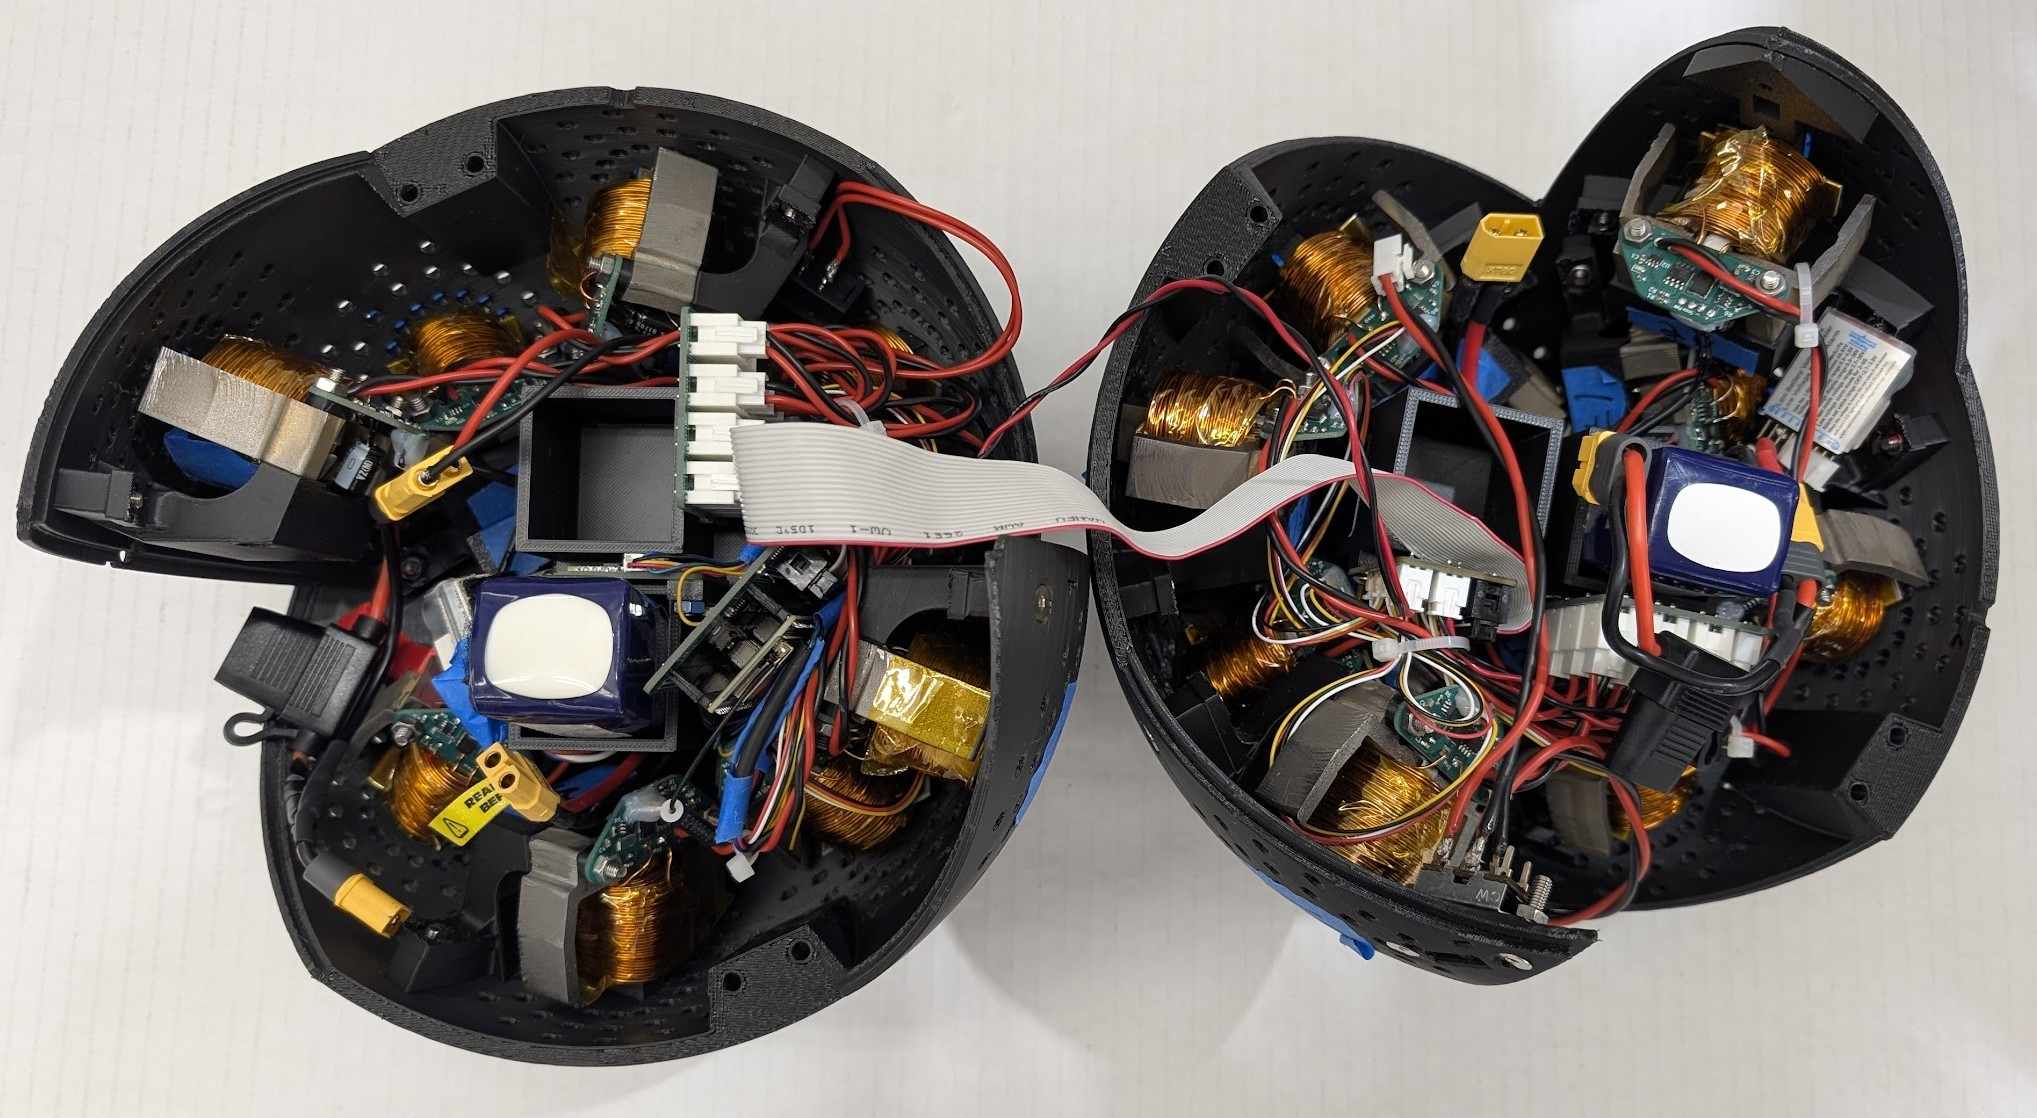
\includegraphics[width=0.8\textwidth]{Diagrams and Images/Full_Ball_Two_Halves.jpg}\\[1cm]
    Josh Bauman\\
    Lucas Henderson\\
    Kristopher Kirkwood\\
    Logan Underwood\\
    Levi Varsanyi\\[1cm]

    Project Sponsors:\\
    Dylan Gunn\\
    Miti Isbasescu\\
    Greg Reid\\[1cm]

    Project 2507\\
    Applied Science 459\\
    Boye Ahlborn Engineering Physics Project Laboratory\\
    The University of British Columbia\\
    April 12, 2025
\end{titlepage}


\newpage
\subsection*{Executive Summary}

An onboard control system, utilizing an inertial measurement unit (IMU) and a state machine algorithm, calculates the real-time orientation of the sphere to dynamically activate the optimal electromagnets for sustained motion.

Transitioning to the 3D geometry introduced significant spatial and weight constraints. While the previous test stand relied on an external power supply, managing the onboard power requirements became a design challenge for the full sphere.

Although the 20-magnet configuration successfully demonstrates the viability of electromagnetic propulsion, system performance is currently limited by its power-to-weight ratio. Testing indicates that to achieve rapid directional changes and higher torque, future iterations will require the integration of higher-capacity batteries and an increased magnet density for a higher resolution of movement.

% Preliminary pages with Roman numerals
\pagenumbering{roman}
\setcounter{page}{2}

% Table of Contents
\newpage
\tableofcontents


% Table of Figures with titles only
\newpage
\renewcommand{\cftfigpresnum}{Figure }
\renewcommand{\cftfigaftersnum}{:}
\renewcommand{\cftfigdotsep}{\cftnodots}
\setlength{\cftfignumwidth}{3cm}
\listoffigures
\newpage

% Main content with Arabic page numbers starting at 1
\pagenumbering{arabic}
\setcounter{page}{1}

% === SECTIONS ===
\newpage

\section{Introduction}
Conventional motors use electrical currents, conductive windings, and magnetic materials in a variety of configurations to produce torque and control the rotation of a rotor. Switched reluctance motors (SRM) like the one shown in Figure \ref{fig:SRM_Diagram}, achieve rotation through a distribution of individually energized stator poles (electromagnets) and a simple ferromagnetic rotor. Torque is produced by sequentially energizing the different stator windings, causing the rotor to attract to the pole. This process exploits the principle of reluctance torque where the rotor naturally seeks a position which minimizes magnetic reluctance.

\begin{figure}[h]
    \centering
    
\includegraphics[width=0.6\textwidth]{Kris_Visuals/SRM_Diagram.png}
    \caption[Switch Reluctance Motor Diagram]{A simplified diagram of a switched reluctance motor consists of a rotating ferromagnetic rotor, and powered stator poles.}
~\label{fig:SRM_Diagram}
\end{figure}

Our sponsor, the Project Lab, challenged our team to invert the traditional concepts of a switched reluctance motor, and design a spherical robot which uses internal electromagnets to generate controlled rolling motion along a ferromagnetic surface. Comparing the operation to an SRM, the stator becomes our robot, and the rotor becomes the ferromagnetic surface which our robot moves along. Torque and therefore motion is produced from the system’s natural tendency to minimize the reluctance (air gap) between the energized electromagnet and the ferromagnetic surface. The electromagnets inside the robot are individually controlled to manage the sphere's position and rotational speed.

As shown in Figure~\ref{fig:Sphere_Torque_Generation}, when an individual electromagnet is powered, it generates a magnetic field (blue), which magnetizes the ferromagnetic surface, resulting in an attractive force downward. The force creates a torque, rotating the ball forward. All necessary electronics, power supplies, sensors, and control devices are contained within the body of the robot. This inverted approach allows us to apply magnetic circuit theory, develop power electronic systems, and implement advanced control algorithms in the context of a challenging and unconventional engineering problem. Concepts drawn from traditional reluctance motors aided in our design, however we did not see any projects similar to this during our research.

\begin{figure}[h]
    \centering
    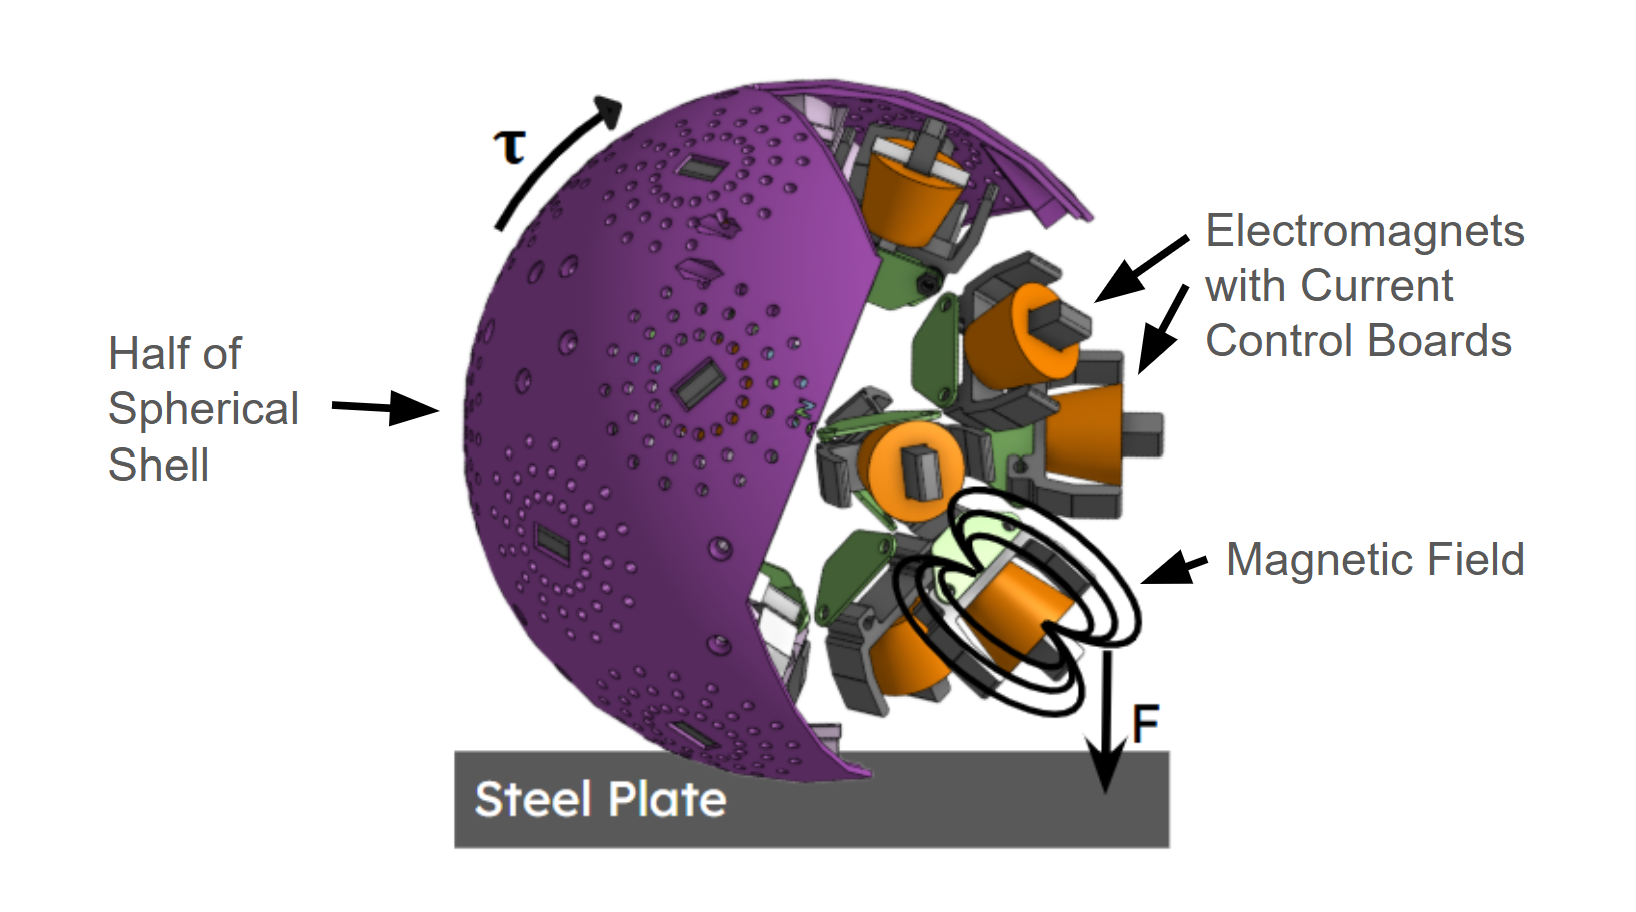
\includegraphics[width=0.8\textwidth]{Kris_Visuals/Ball_torque_image2.png}
    \caption[Torque Generation of Sphere]{The electromagnets around the ball create an attractive force to the ferromagnetic surface (orange arrow), resulting in a rotation about its center (red arrow)}
    \label{fig:Sphere_Torque_Generation}
\end{figure}

To reduce project risk and aid in early-stage design, we focused our initial efforts on developing a simplified physical prototype: a disk that rotates on a fixed test stand above a ferromagnetic plate. This allowed us to focus on validating magnet designs, build and test the driving electronics, and prototype control software in a more manageable, two-dimensional setup. For more information on last year’s prototype, see the Project 2507 report~\cite{2507_report}.

Building on our previous work, this year we focused on system design, manufacturing, integration, and control. An optimal magnet design was chosen and twenty cores and coils were manufactured, along with twenty identical current control circuits. These isolated electromagnet subsystems were then integrated into a spherical shell geometry, along with the intertial measurement unit (IMU), microcontroller, and batteries. A control architecture was developed to use the IMU data to determine the sphere’s orientation and activate the appropriate electromagnets to maintain motion. Finally, we tested the system’s performance and identified key areas for improvement in future iterations.

\section{Discussion}
\subsection{System Level Overview}

\begin{figure}[h]
    \centering
    
\includegraphics[width=0.5\textwidth]{Diagrams and Images/work_in_progress.png}
    \caption[System level Diagram]{Overview of our system}
    \label{fig:SLD}
\end{figure}


By breaking the system down into these components, we were able to design and test each one in isolation. This modular approach allowed us to develop the electromagnets independently, while creating and refining the driving circuit in parallel.

\subsection{Electromagnet}
\subsubsection{Theory}


\begin{figure}[H]
    \centering
    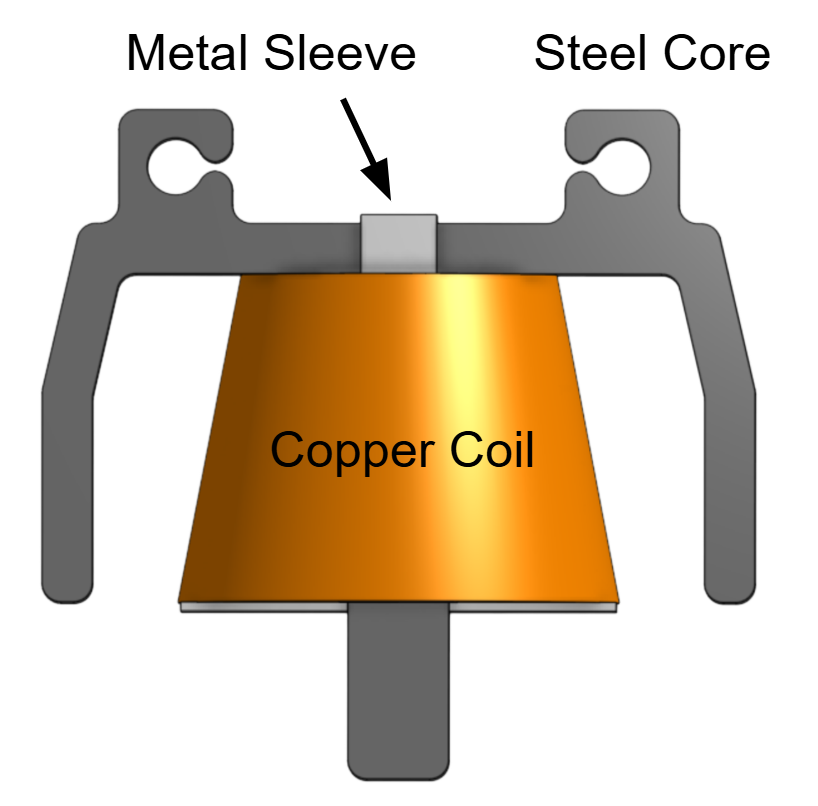
\includegraphics[width=0.4\textwidth]{Kris_Visuals/2026_Magnet_CAD.png}
    \caption[2026 Magnet Design]{The final design of our electromagnets, which we found to be the most effective in testing.}\label{fig:2026_magnet_design}
\end{figure}

\subsubsection{Core Design}
TODO: Delete at end.

\subsubsection{Manufacturing}\label{sec: mag manufacturing}

\subsection{Magnet Driver Electronics}

\subsubsection{High Level Architecture}
The attractive force produced by a given electromagnet is directly related to the current flowing through it, so independent control of the current in each electromagnet is necessary to achieve intelligent force modulation and control over the motion of the ball. 

Electrically, the electromagnets can be modelled as a series combination of a resistance $R$ and an inductance $L$. When a voltage is applied across an electromagnet, the current through it rises with an RL exponential characteristic and when the voltage is removed, the current falls with a similar characteristic. By rapidly switching the applied voltage on and off (with MOSFET), the current can be shaped to achieve a desired average value, forming the basis of our current control strategy. Figure \ref{fig:exampleCurrent} illustrates an example electromagnet current waveform with switching driven by a PWM signal.

\begin{figure}[H]
    \centering
    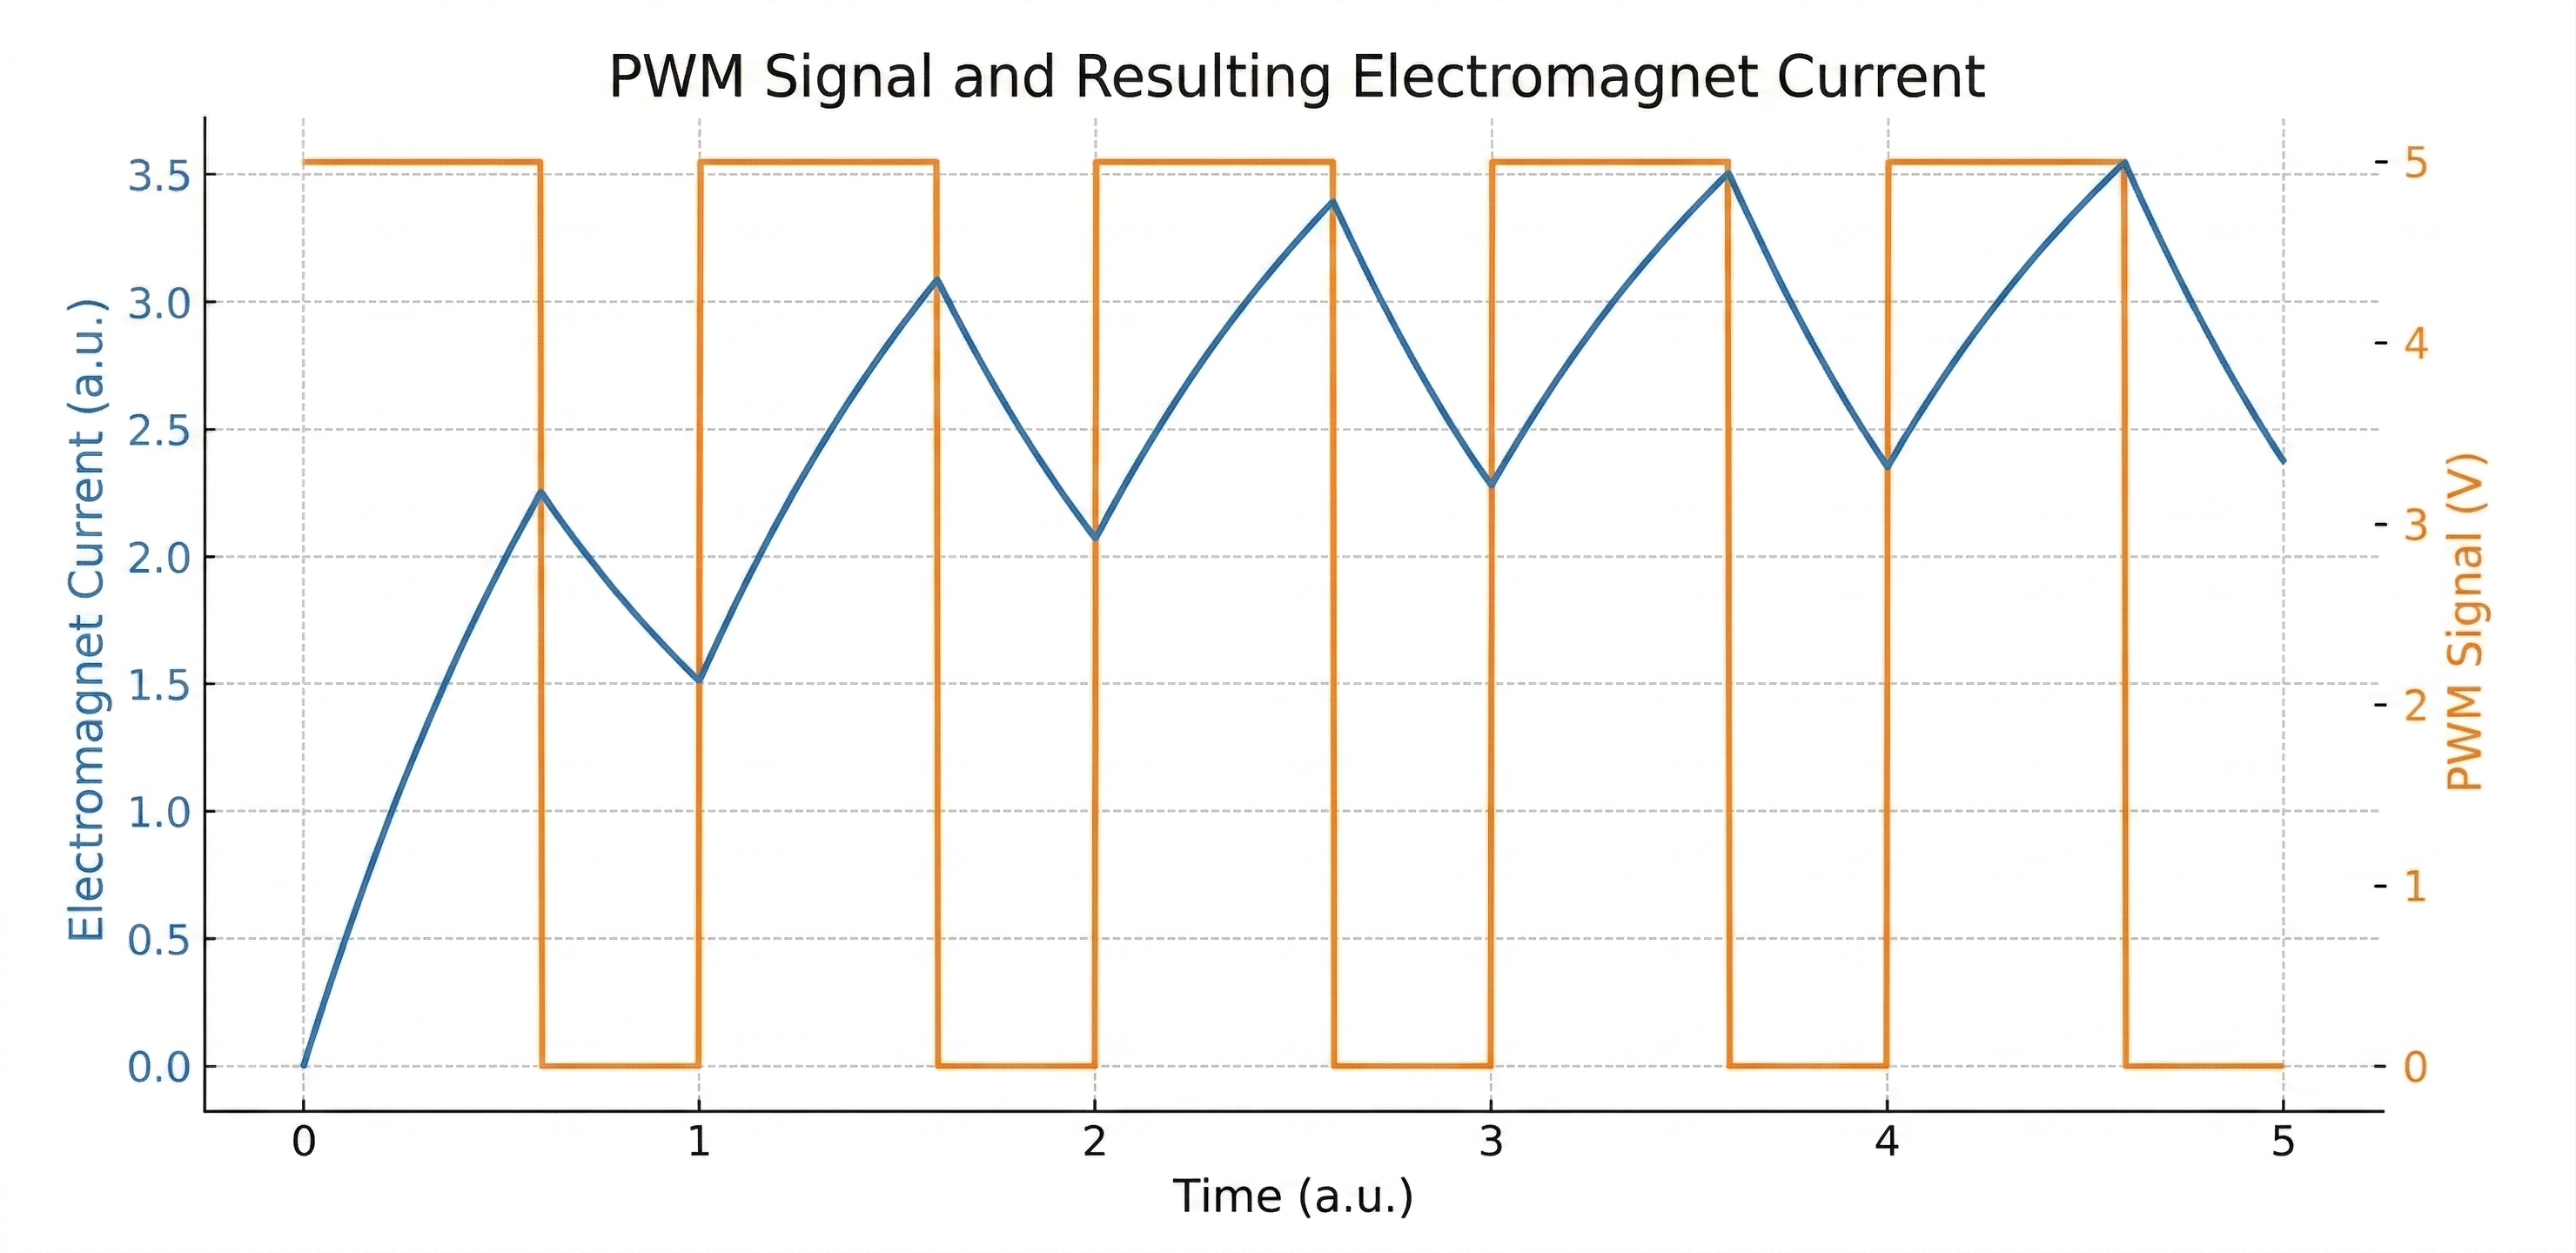
\includegraphics[width=0.7\textwidth]{Diagrams and Images/exampleElectromagnetCurrent.png}
    \caption[exampleCurrent]{Illustrative example of the current through an electromagnet as it is modulated through the switching of an applied voltage. When the switch is closed, the current rises with an RL exponential characteristic, and when the switch is opened, the current falls an RL exponential characteristic. The average current can be modulated by changing the duty cycle of the PWM signal, and the current ripple can be reduced by increasing the PWM switching frequency. The ripple in this example is exaggerated for illustrative purposes, but in practice with switching at frequencies in the 10's of kHz, ripple can be reduced to less than a few percent of the average current.}
    \label{fig:exampleCurrent}
\end{figure}

Figure \ref{fig:Schematic} shows the high level architecture used to implement this control strategy. The switching of current through an electromagnet can give rise to large voltage spikes due to inductor kickback if not handled properly. A 'flyback' diode is used to provide a path for the electromagnet current to discharge safely when the switch is opened, and to also avoid abrupt drops in current which would otherwise degrade controllability. Furthermore, the instantaneous current through the electromagnet is monitored using a shunt resistor and differential amplifier, providing feedback for closed-loop control of the current. Based on this current measurement and the desired current, an ESP32 modulates the duty cycle of the MOSFET gate PWM signal to achieve the target current. 

\begin{figure}[H]
    \centering
    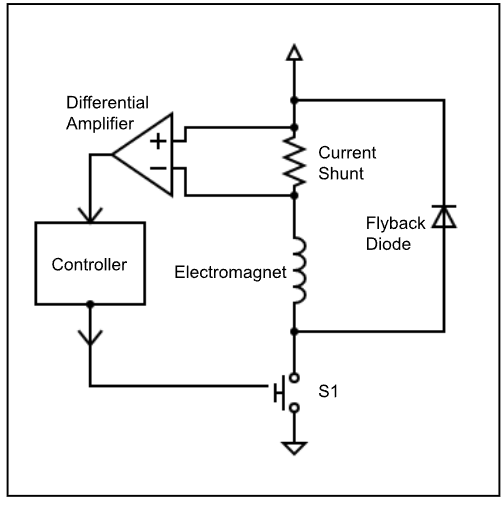
\includegraphics[width=0.4\textwidth]{Circuit Visuals/Circuit Schematic.png}
    \caption[Schematic]{High-level architecture of the electromagnet current driver circuit}
    \label{fig:Schematic}
\end{figure}

\subsubsection{Design}
The final schematic for the implementation of the current driver is shown in Figure \ref{fig:kiCadSchematic}.


\begin{figure}[H]
    \centering
    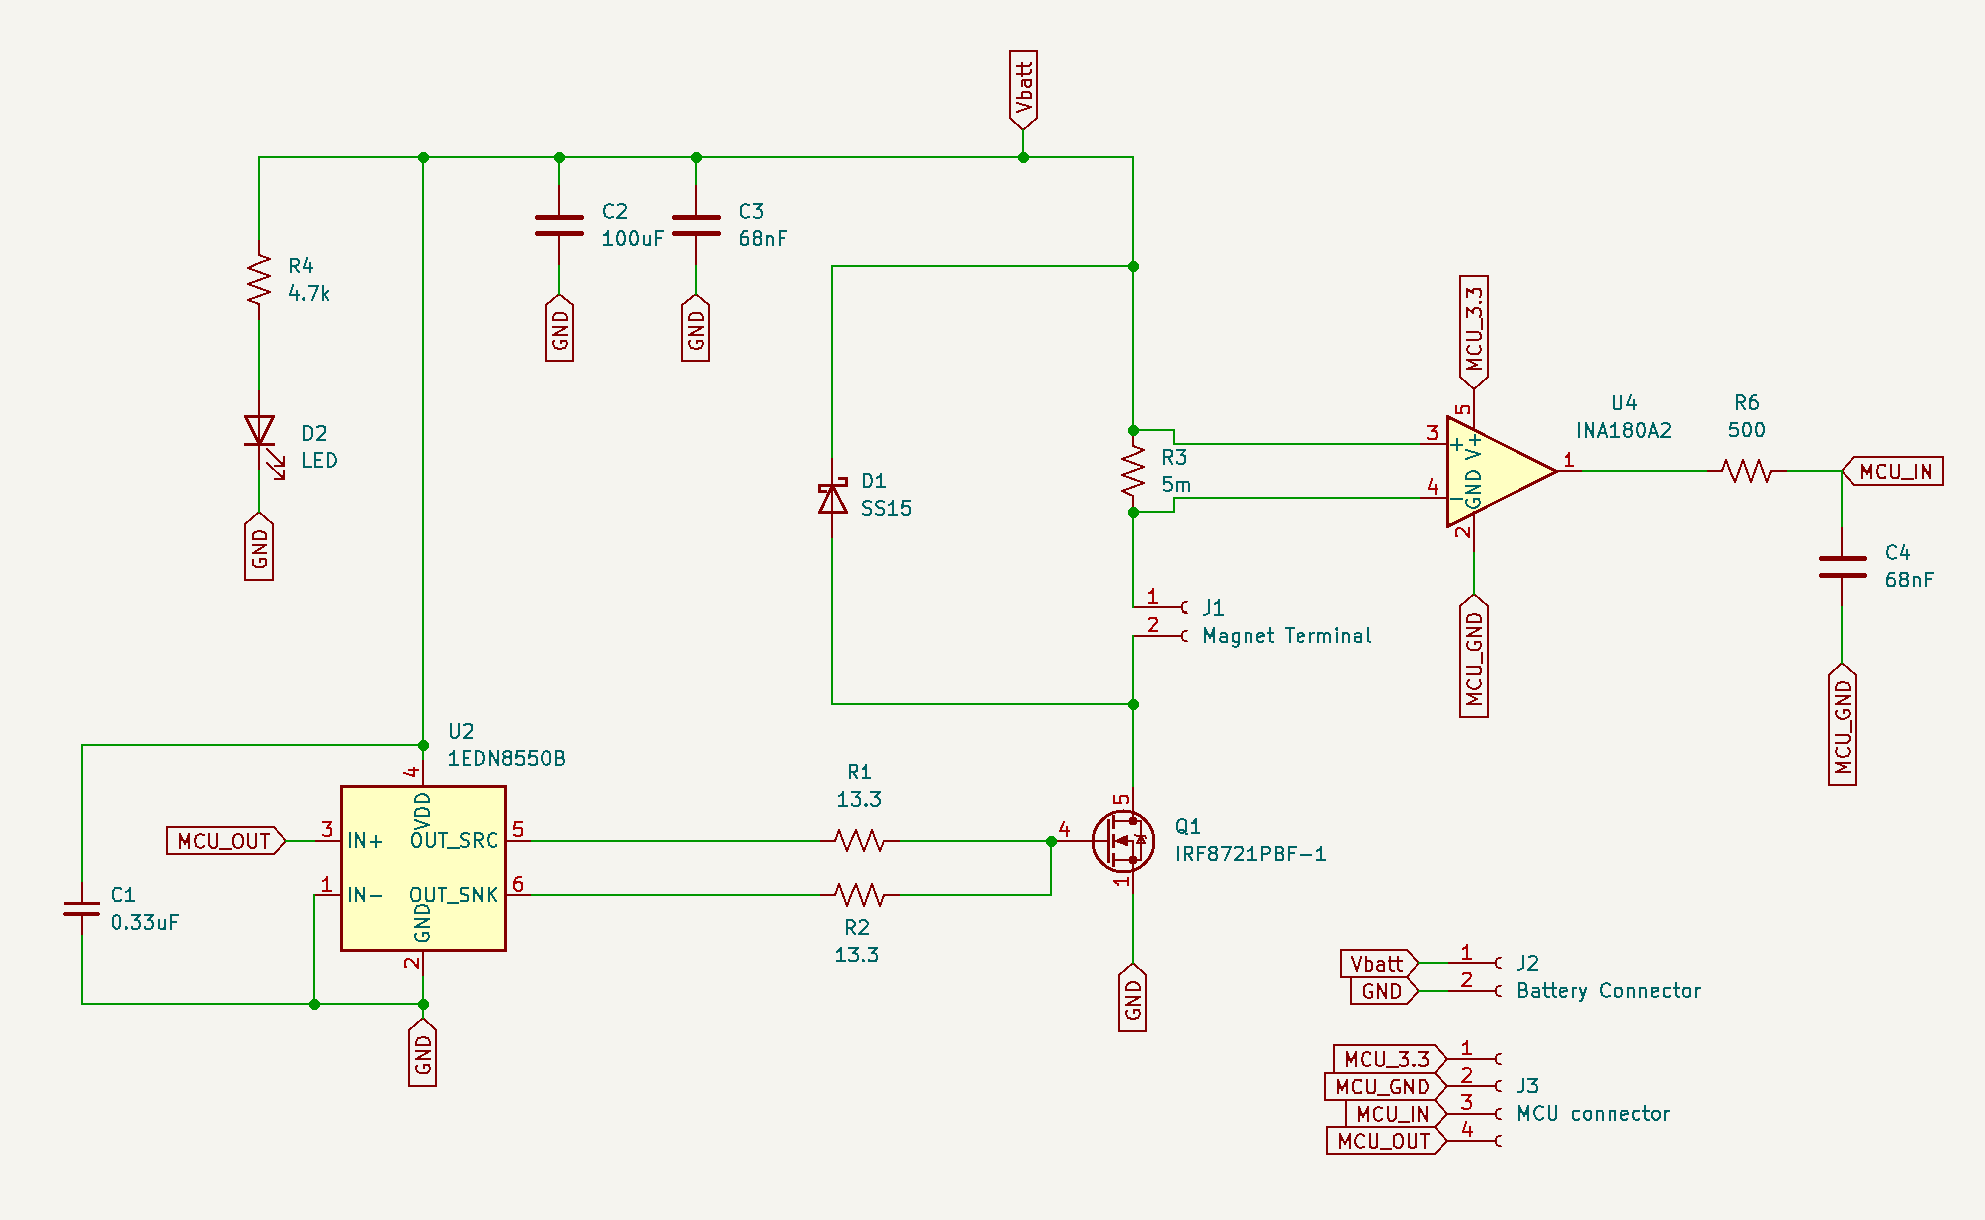
\includegraphics[width=0.7\textwidth]{Diagrams and Images/driverSchematicKiCad.png}
    \caption[Schematic]{Final KiCad Schematic for electromagnet current driver circuit}
    \label{fig:kiCadSchematic}
\end{figure}

\textbf{Switching Stage}\\
A gate driver is used to drive the gate of the MOSFET, providing the necessary voltage and current to charge and discharge the gate capacitance quickly, reducing switching losses in the MOSFET. This fast switching allows for higher PWM frequencies, which reduces current ripple, while maintaining tolerable heat dissipation. On turn off events, there is some finite time that the flyback diode takes to conduct and allow the current to discharge. For very fast switching speeds, this can lead to a large drain-source voltage overshoot that can damage the MOSFET. To mitigate this, we limit the switching speed using gate resistors which limit the gate charging current. Figure \ref{fig:gateResComparison}, shows the effect of increasing the gate resistance from 1 $\Omega$ to 13.3 $\Omega$. The effect is to bring the voltage overshoot down from the near the MOSFET's maximum drain-source voltage rating of 30 V to a safe level.

\begin{figure}[H]
    \centering
    \begin{subfigure}[t]{0.48\textwidth}
        \centering
        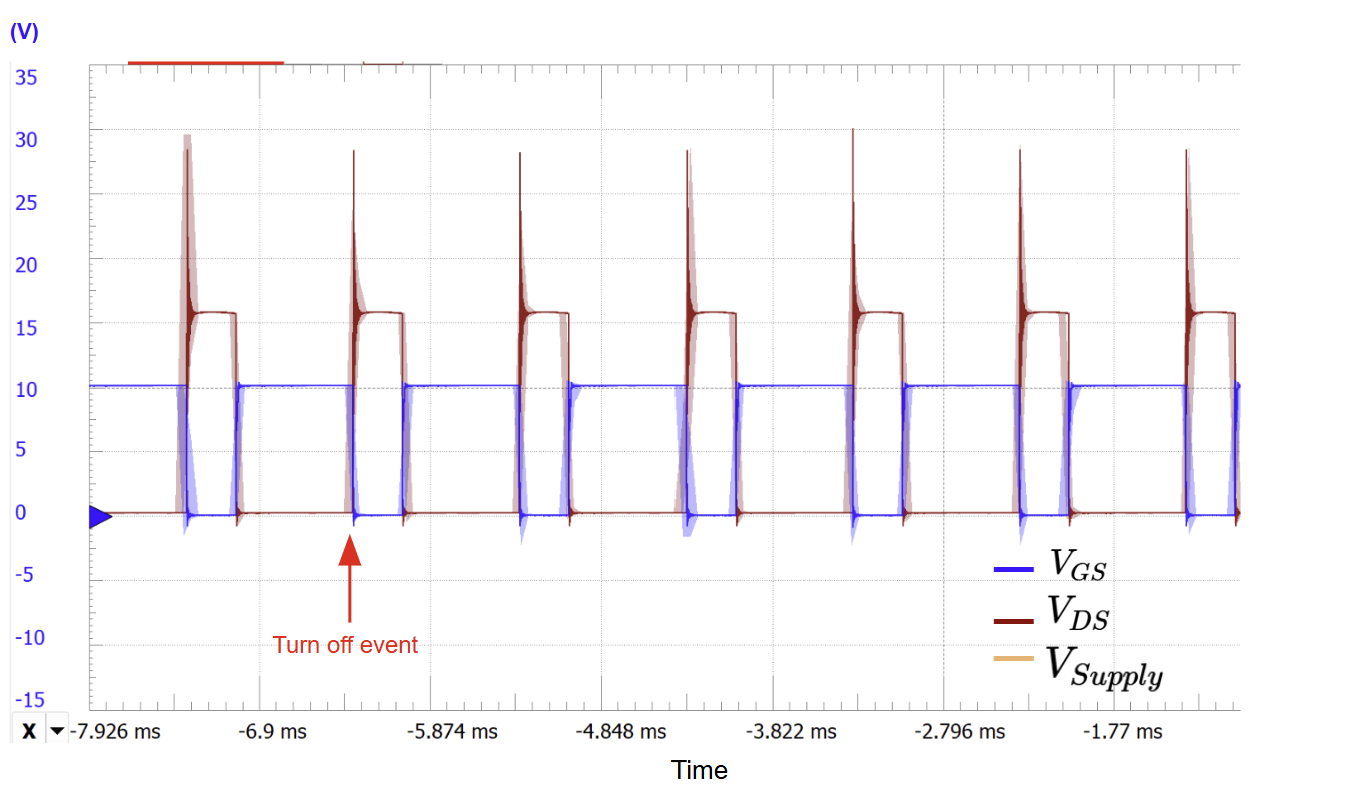
\includegraphics[width=\textwidth]{Diagrams and Images/withoutGateRes.png}
        \caption{1 $\Omega$ gate resistance}
        \label{fig:withoutGateRes}
    \end{subfigure}
    \hfill
    \begin{subfigure}[t]{0.48\textwidth}
        \centering
        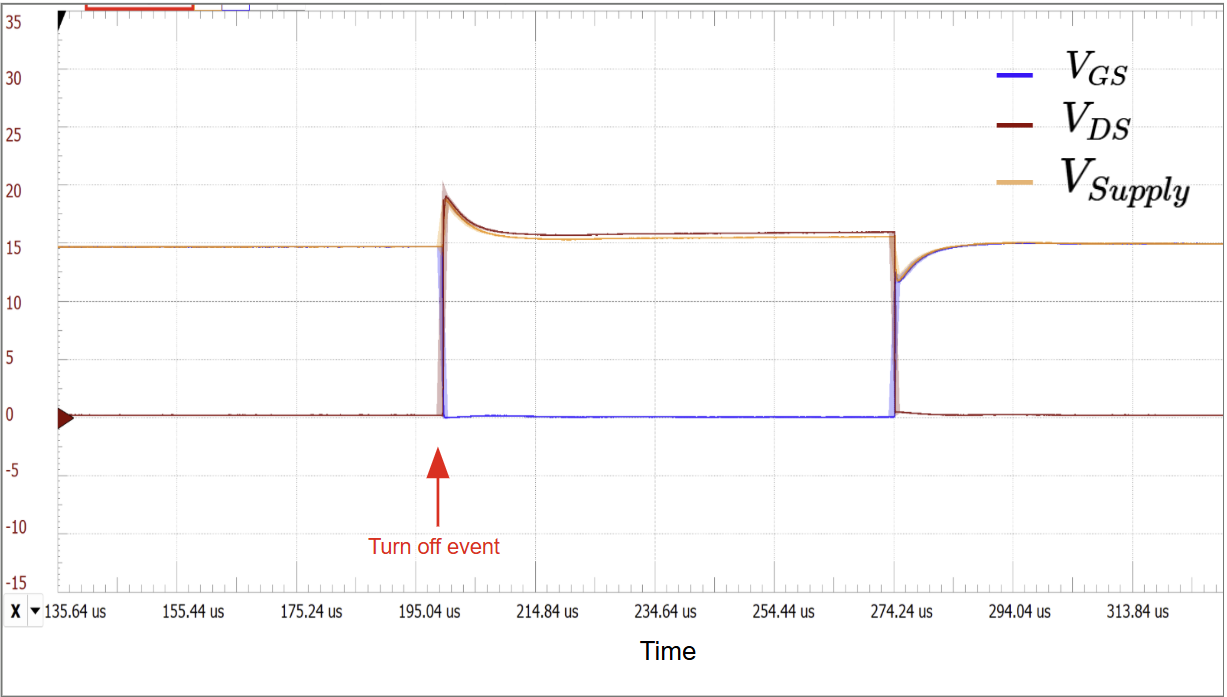
\includegraphics[width=\textwidth]{Diagrams and Images/withGateRes.png}
        \caption{13.3 $\Omega$ gate resistance}
        \label{fig:withGateRes}
    \end{subfigure}
    \caption{Drain-source voltage overshoot on turn off events with different gate resistance values. The gate resistors limit the switching speed of the MOSFET, which reduces the voltage overshoot and protects the MOSFET from damage.}
    \label{fig:gateResComparison}
\end{figure}


\textbf{Current Sensing}\\
The shunt resistor and differential amplifier are selected to provide optimal accuracy and resolution. A 5 m$\Omega$ shunt was selected to keep power loss small. Care was taken to select a shunt resistor with low parasitic inductance to minimize di/dt noise in the current measurement. A TI INA180 current sense amplifer was selected having a gain of 50 V/V giving a measureable current range of 0-13.2 A with its 3.3 V output range. An RC lowpass filter with 5 kHz cuttoff is used on the output to attenuate high frequency switching noise before the signal is given to the ADC.

\textbf{Power}\\
Each current driver requires two voltage supply levels to support its operation. The electromagnets must be supplied with high enough voltage to deliver currents up to 10A (based on magnet testing and determined magnet force requirements) through a ${\sim}1\,\Omega$ load (electromagnet series resistance). Additionally a higher supply voltage will increase the rate at which current can rise and fall through the electromagnets, improving responsiveness. To balance battery size and performance, a 14.7 V rail was determined to be sufficient. 

A 3.3 V supply is also required to power the current sense amplifier. This is supplied by the ESP32's internal voltage regulator, to ensure proper referenceing between the amplifier and the microcontroller. In this driver architecture, the gate drive is supplied with the same 14.7 V supply as the electromagnets. When the electromagnets pull current, stray inductance between the magnet terminal and the battery leads cause the supply voltage to sag. If the supply sags too low, the gate driver may enter a lock-out mode, preventing it from driving the MOSFET. A sag in supply voltage also degrades the performance of the current driver since the electromagnet is being driven with a lower voltage. To solve this issue, a large 100 $\mu$F electrolytic capacitor is placed across the supply rails on the current driver board to provide a local charge reservoir for the current driver to source current from. A small 68 $nF$ ceramic capacitor is placed in parallel to the electrolytic to filter out high frequency noise on the supply.

Figure \ref{fig:unitCellDiagram} shows the final unit cell magnet actuator, which includes the electromagnet, current driver, and connections to the microcontroller and power supply.

\begin{figure}[H]
    \centering
    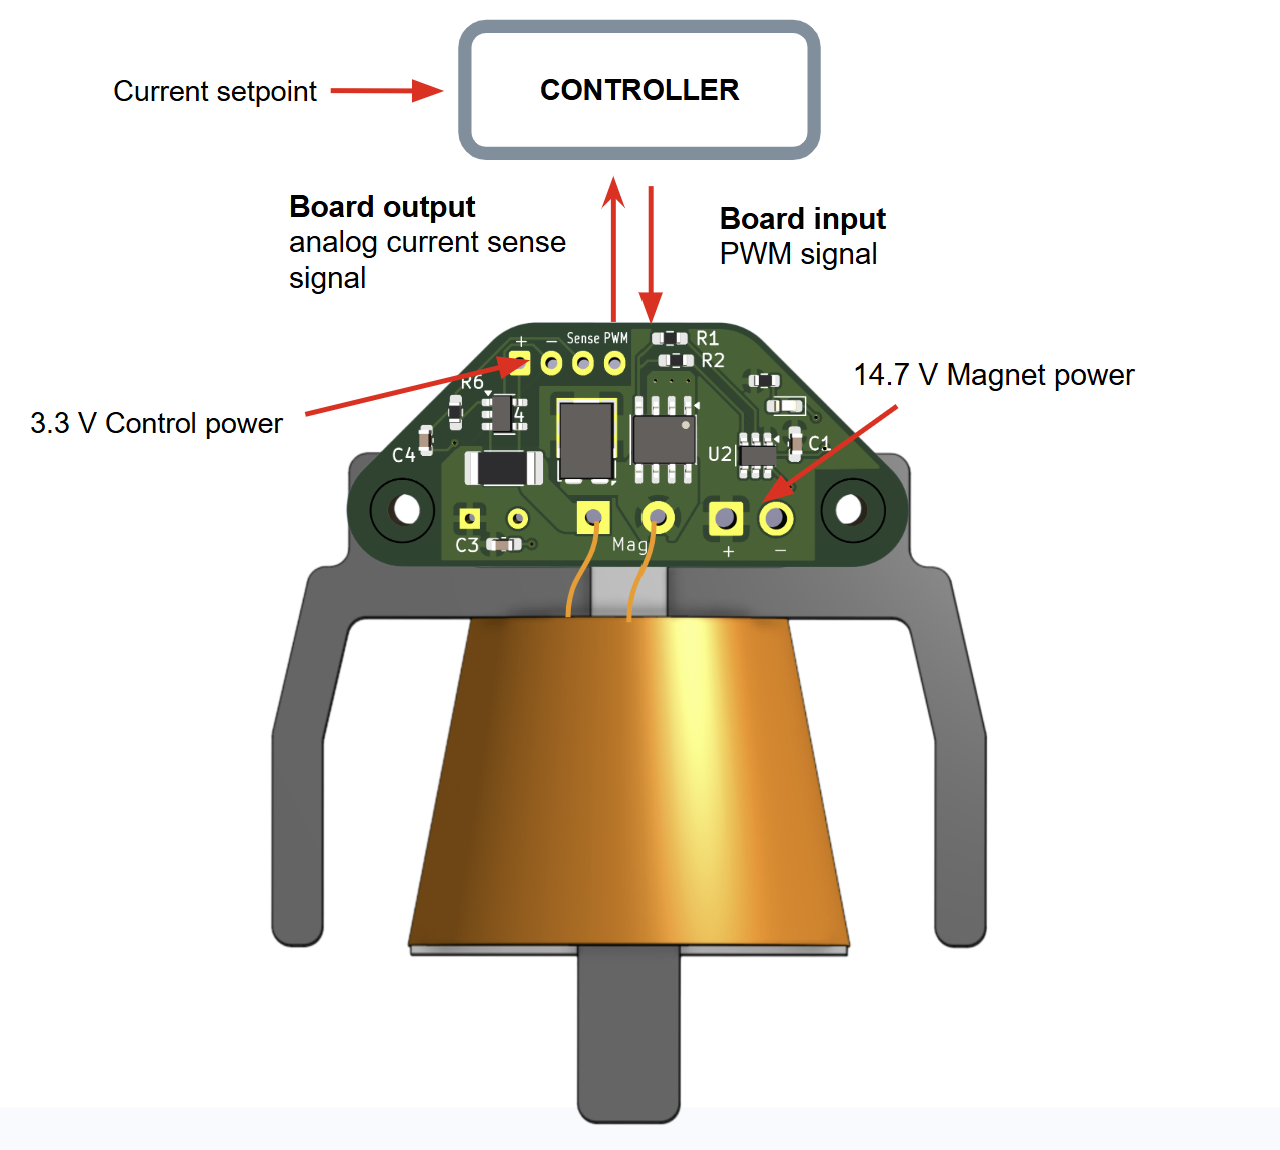
\includegraphics[width=0.8\textwidth]{Diagrams and Images/unitCellDiagram.png}
    \caption[PCB]{Unit cell magnet actuator. PWM signal from microcontroller is input to the current driver board. Analog current sense signal is sent to ADC on microcontroller board creating closed loop feedback scheme. 14.7 V battery supply is used to power the electromagnet, and 3.3 V supplied from microcontroller is used to power the current sense amplifier.}\label{fig:unitCellDiagram}
\end{figure}


\subsection{Software Architecture}
The software systems connects all system components allowing the system to function. This section will discuss the high level goals of the system and will discuss some of the implementation details of the system. 

\subsubsection{Background}
The high level goal of the software is to cooridnate the current going throiugh each magnet to deliver motion in a desired direction indicated by the joystick. To accomplish this, the software must be able to determine the: location of each magnet relative to the origin of the ball, selection of which magnet to activiate, and calibration between the joystick and the ball. 

\begin{figure}[h]
    \centering
    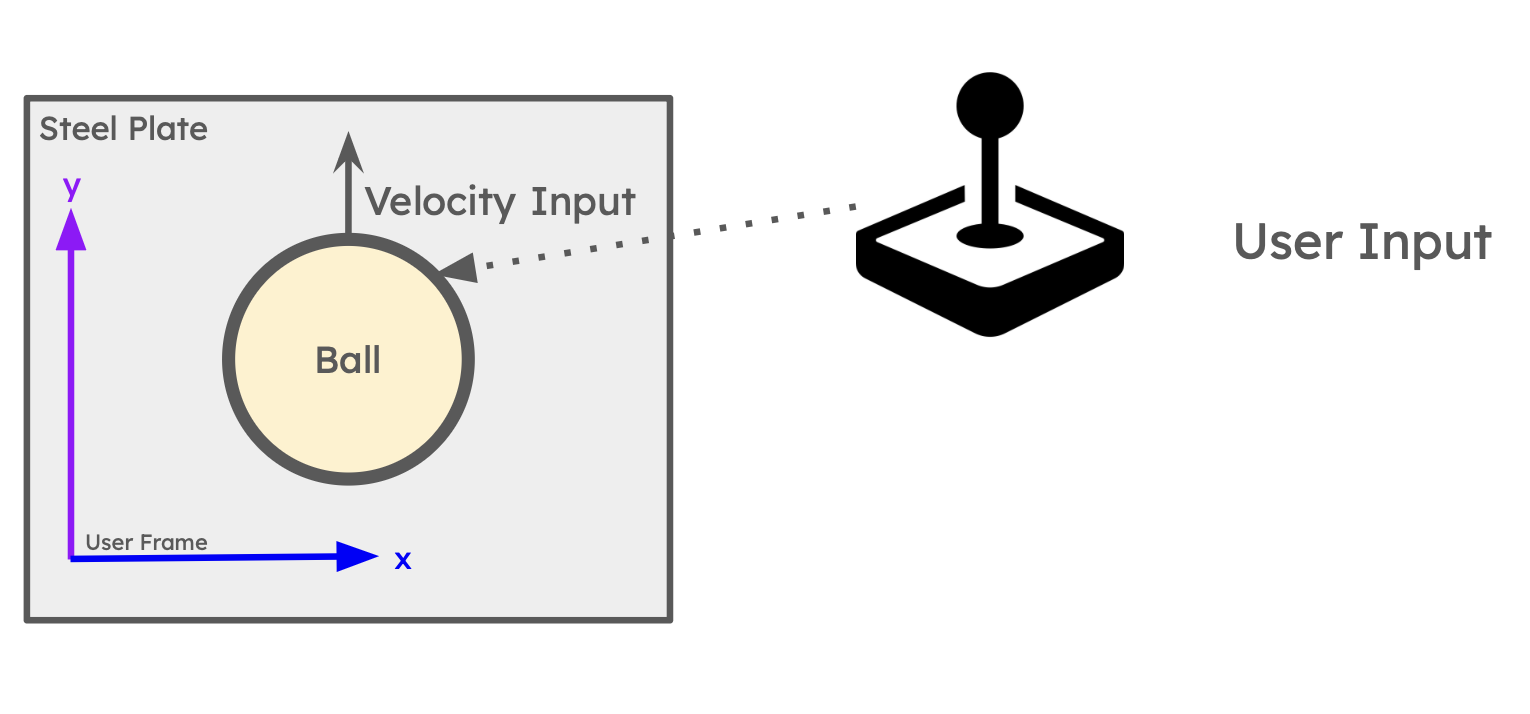
\includegraphics[width=0.75\textwidth]{Diagrams and Images/eye-of-god-figure.png}
    \caption[Software Overview]{A diagram outlining the functionality hoping to be achieved by the software.}
    \label{fig:Software_Overview}
\end{figure}

The software will be running on the ball and our dashboard interfacing together to create a cohesive experince for the user. 


\subsubsection{Data Communication Overview}
The first important challenge is to figure out how the different components of our system will interact and pass data in between. Since our ball will rotate omnidirectionally, a wired data trasmission makes little sense. We choose to implement a wifi based communication hosted on the ESP that the dahsboard would connect to. 

\begin{figure}
    \centering
    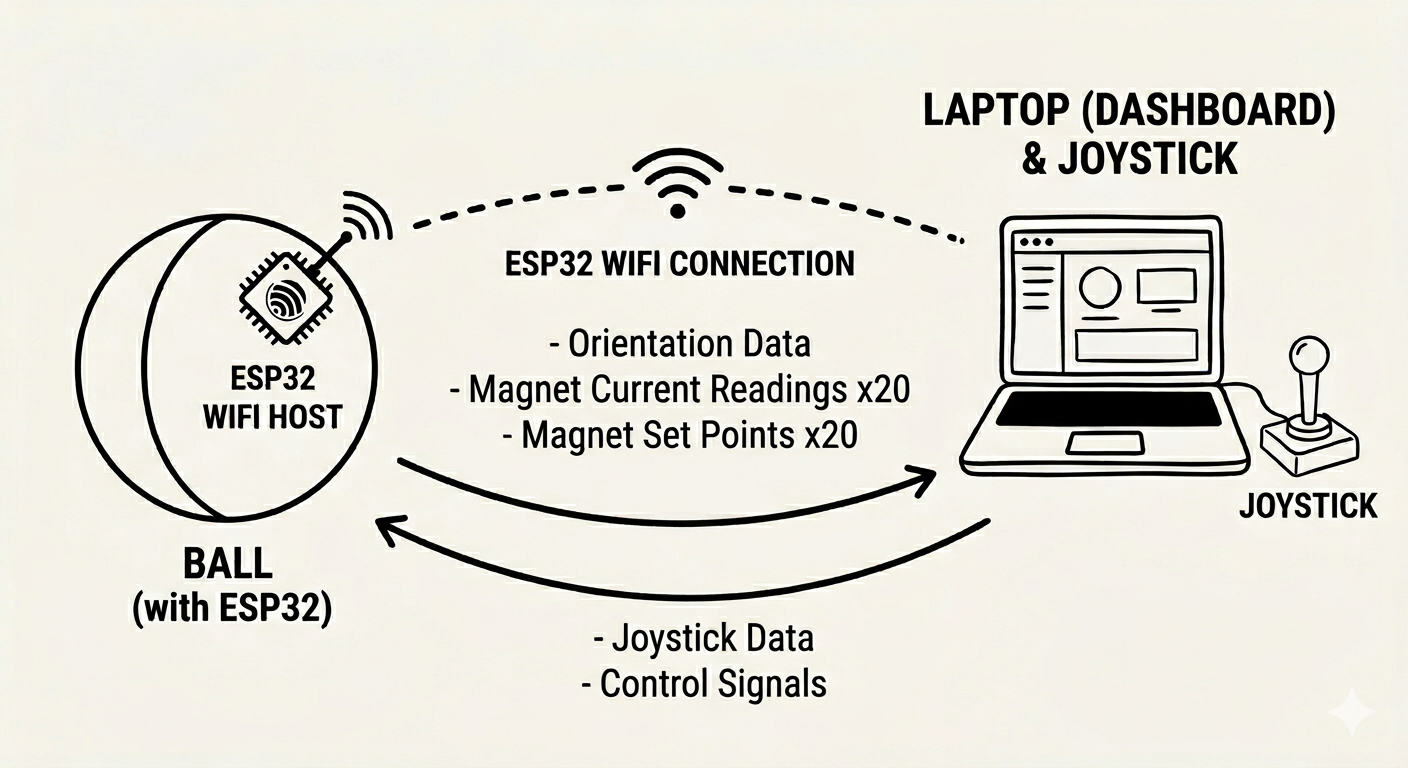
\includegraphics[width=0.75\textwidth]{Diagrams and Images/communication-diagram.png}
    \caption[Communication Diagram]{A diagram outlining the communication between the user interface and the ball.}
    \label{fig:Communication_Diagram}
\end{figure}

Our outgoing data packet size was $276$ bytes which communicated when communicated at a rate of $10 \: \text{Hz}$ gives us a data rate of $2.76 \frac{\text{kB}}{\text{s}}$ which is well within the capabilities of a wifi connection. Inbound data to the ESP is minimal and consiting a few bytes at sporatic intervals, so we do not experience any issues with the data rate in the incoming direction.

\subsubsection{State Machine}
Our on device state management is implemeneted as a state machine. An outline of the state machine is shown in Figure \ref{fig:State_Machine}. 

\begin{figure}[h]
    \centering
    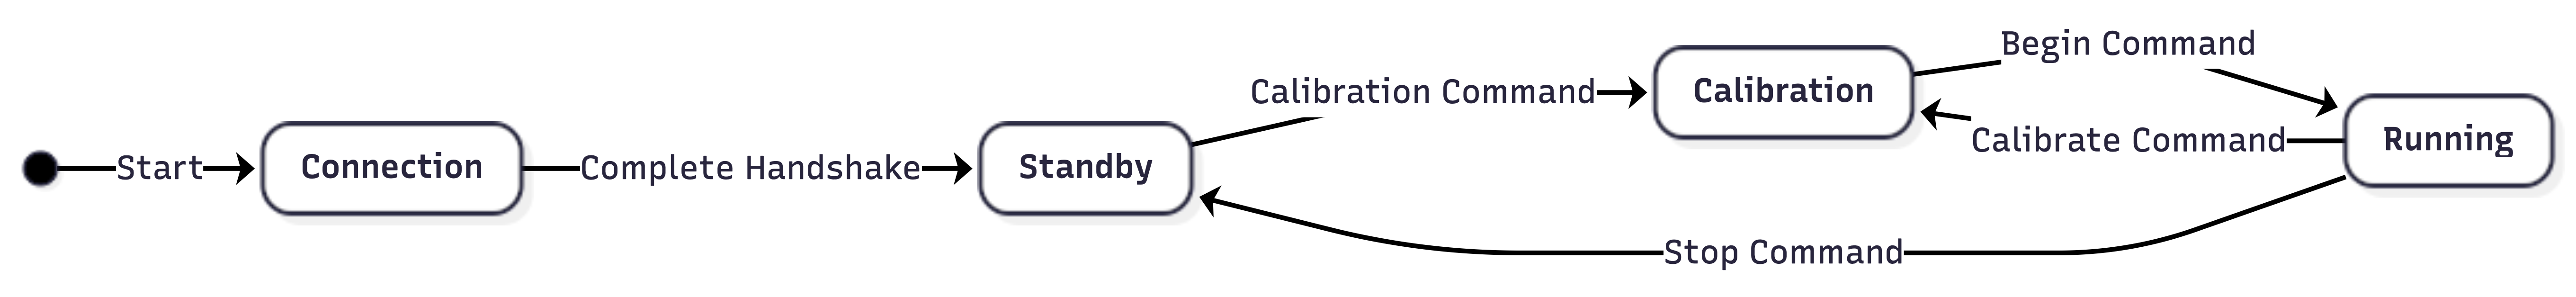
\includegraphics[width=1.0\textwidth]{Diagrams and Images/state-machine-breakdown.png}
    \caption[State Machine Diagram]{Outline of the state machine implemented on the microcontroller.}
    \label{fig:State_Machine}
\end{figure}

Each state corresponds to a different mode of operation for the device, details on each is outlined below:
\begin{itemize}
    \item \textbf{Connection}: The device waits for a handshake from the user interface. 
    \item \textbf{Standby}: The device is connected and waits for a command to start the calibration process.
    \item \textbf{Calibration}: The device performs a calibration routine communicating with the user interface (more detail found in Section \ref{sec:calibration}).
    \item \textbf{Active}: The device is actively controlling the electromagnets to move the ball according to user input (more detail found in Section \ref{sec:active}).
\end{itemize}

\subsubsection{Orientation Tracking}
A critical task in our software stack is the ability to track the orientation of the ball. This step is critical becuase this is what tells where each electromagnet is relative to the origin of the ball and this allows us to determine which magnet will need to be activated. Stated simply, we need a way to track the rotational state of the ball.

There are a couple of popular methods for rotation tracking, 2 common approaches (Euler angles and quaternions) are outlined in Figure \ref{fig:angle_tracking_options}. We chose to implement the quaternion approach since it does not suffer from gimbal lock and it more computational effiecent to compute new magnet locations (see \ref{eqn:magnet_rotation}) than the Euler angle approach. For more detail on quaternions see appendix (TODO: add section of quaternions).
\begin{figure}[h]
    \begin{minipage}{0.49\textwidth}
        \centering
        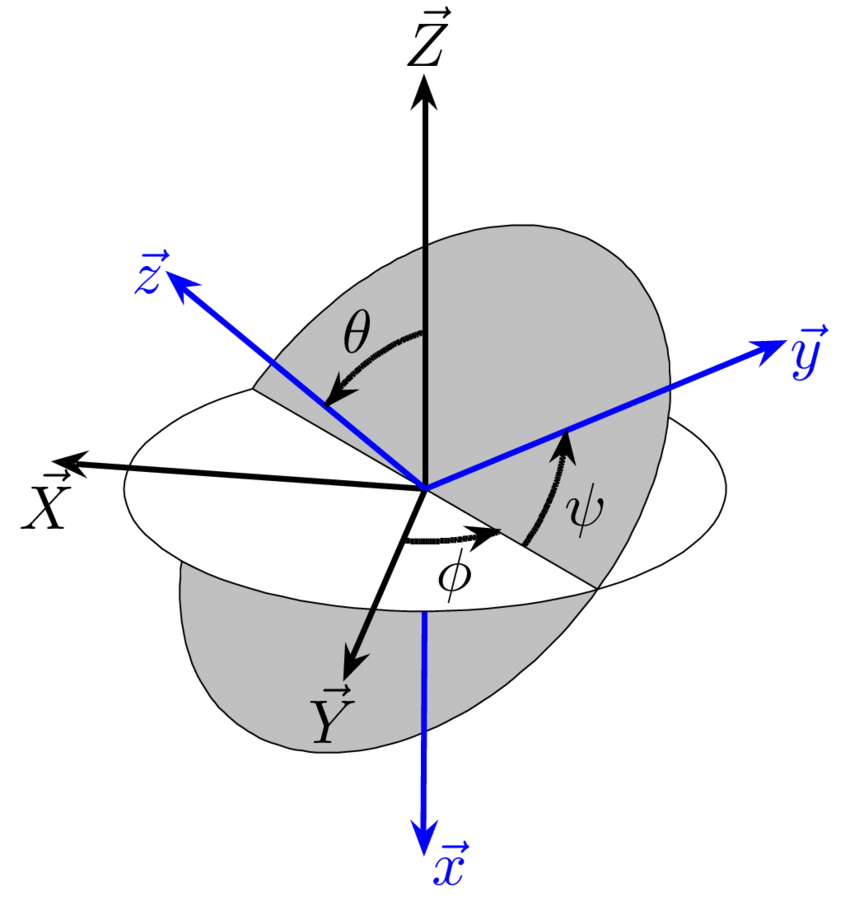
\includegraphics[width=0.98\textwidth]{Diagrams and Images/euler-angle.png}
        \caption[Euler Angle]{Euler angles is a common representation of rotation that uses three angles to represent the orientation of an object.}
    \end{minipage} 
    \hfill
    \begin{minipage}{0.49\textwidth}
        \centering
        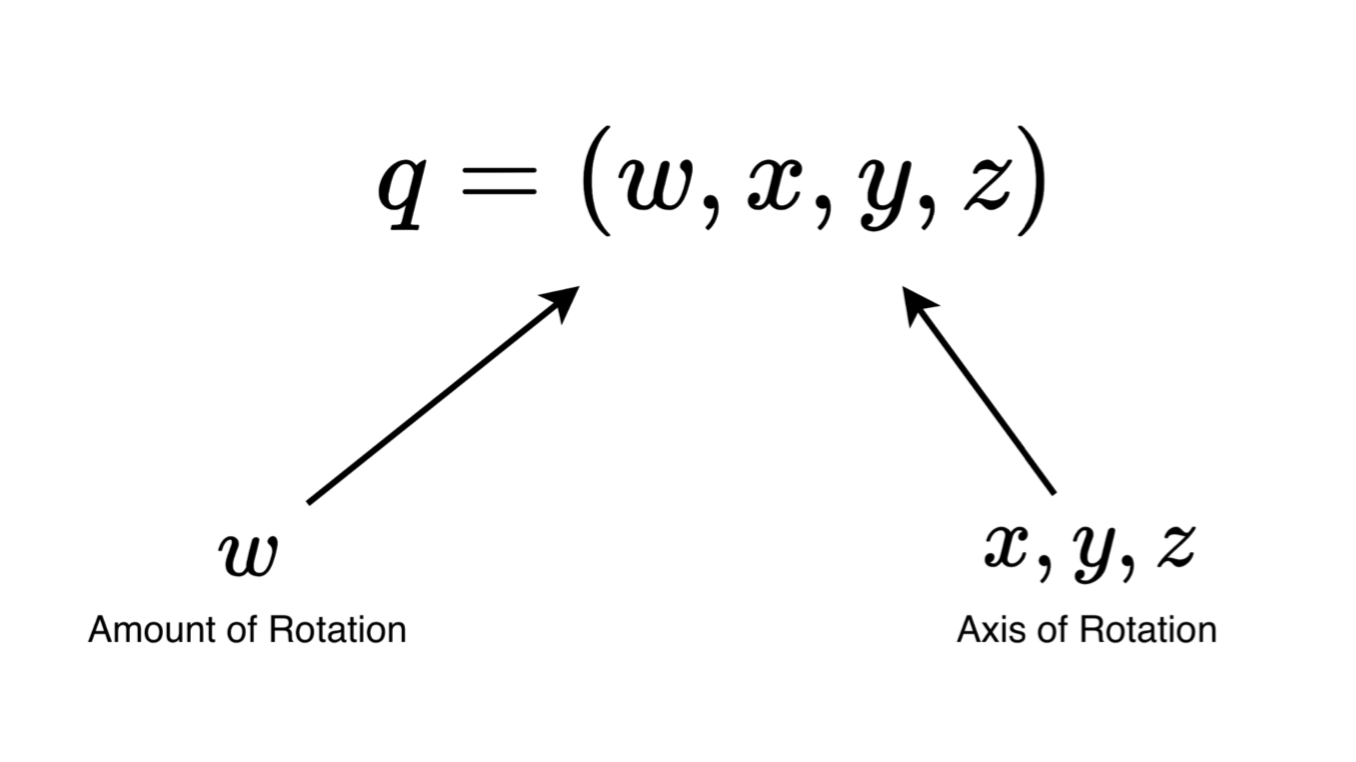
\includegraphics[width=0.98\textwidth]{Diagrams and Images/quaternion-basics.png}
        \caption[Quaternion]{A quaternion is a mathematical object similar to a vector of size 4 that can represent the orientation of an object in 3D space.}
    \end{minipage}
    \label{fig:angle_tracking_options}
\end{figure}

An interntial measurment unit (IMU) can be used to update the rotation quaternion $q$ in real time. The quaternion can be calculated by using a famous Madgwick sensor fusion algorithm which combines the data from the accelerometer, gyroscope, and magnetometer outputting a quaternion representing the current state of the ball \cite{Madgwick_2010}. You can learn more about our selection of the IMU in \ref{sec:IMU_selection}

With the quaternion representing the current orientation of the ball, we can determine the location of the magnets relative to the origin of the ball. Critically using the quaternion allows us to map the coordinates of the magnets in the ball’s reference frame to the world reference frame, which is critical allows to align the magnet locations with the joystick input. The rotation of a vector $\vec{v}$ by a quaternion $q$ can be calculated using the following formula:

\begin{equation}
    \vec{v}_{\text{rotated}} = q \vec{v} q^{-1}
    \label{eqn:magnet_rotation}
\end{equation}

By utilizing the above formula and the known locations of the magnets in the ball's reference frame we are able to determine the location of each magnet in the world reference frame. 

\begin{equation}
    \begin{aligned}
        \mathbf{V}_{\text{magnet, world}} &= \begin{bmatrix}
            \vec{v}_{1,\text{world}} \\
            \vdots \\
            \vec{v}_{20,\text{world}}
        \end{bmatrix}, \\
        \vec{v}_{i,\text{world}} &= q\,\vec{v}_{i, \text{ball}}\,q^{-1}, \quad i=1,\ldots,20
    \end{aligned}
    \label{eqn:magnet_world_location}
\end{equation}

\subsubsection*{IMU Selection}
\label{sec:IMU_selection}
There were severel IMU options we considered for this project. We ultimetely selected the FSM300, a 9 degree of freedom IMU with an integrated chip that preforms the Madgwick sensor fusion on device. 

Our IMU selection was determined using a stable drift test. In this test, we placed the IMU on a stable surface and recorded the output quaternion over 5 minutes. We found that the FSM300 had a $10^5$ times lower drift than the BN09X (the cheaper alternative).  

\subsubsection{Magnet Selection}
\label{sec:magnet_selection}
TODO (left for LEVI)

\subsubsection{Magnet Current Control}
\label{sec:magnet_current_control}
(TODO fill out later Logan)

\subsubsection{Active State}
\label{sec:active}
In the active state, our ESP runs to seperate processes, one on each core on the esp. One core is responable for receiving and sending data to the dashboard. The other core is responsible for the orientation tracking, magnet selection, and magnet current control. 

The two cores communicate through a globally shared object that contains the current state of the system. All shared memory is protected by mutexes to prevent race conditions between cores. More detail on the shared data between cores can be found in (appendix TODO: add section on shared data).

\begin{figure}[h]
    \centering
    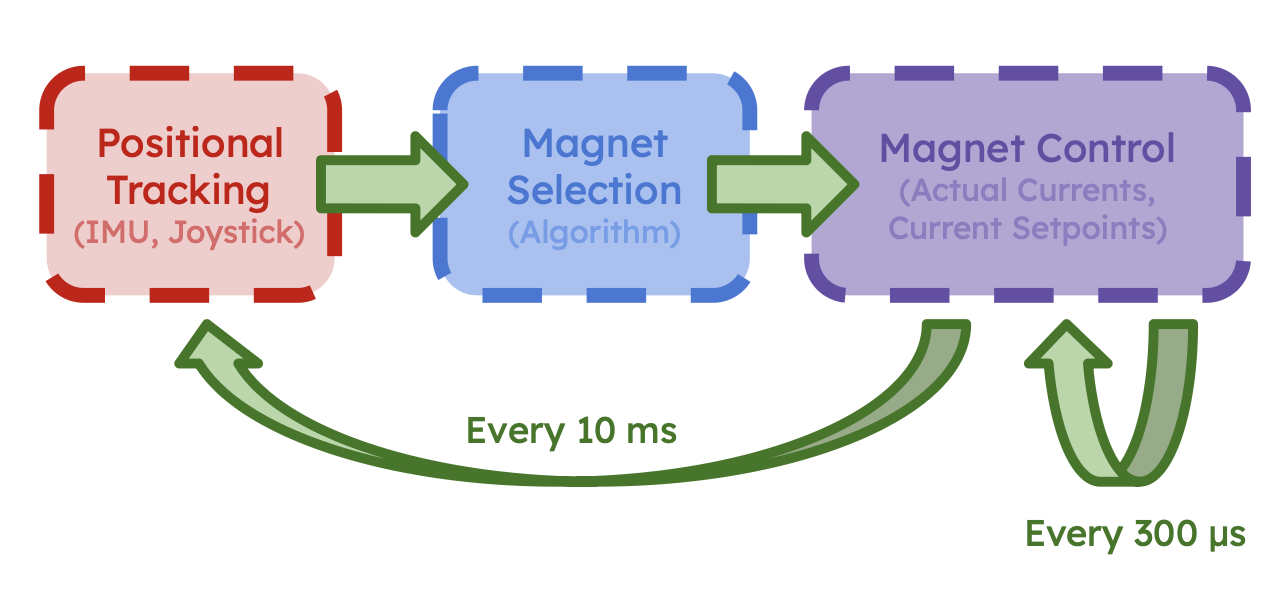
\includegraphics[width=0.75\textwidth]{Diagrams and Images/core-1-loop.png}
    \caption[Active State Diagram]{A diagram outlining the control flow in core 1 loop during the active state.}
    \label{fig:Active_State_Diagram}
\end{figure}

The control loop is run on core 1 with the watchdog turned off to allow us to run our fast loop at $3.33 \text{KHz}$. Every 10 milliseconds, the algorithm checks for new orientation data from the IMU. The magnet selection algorothm runs using the new locations of each magnet in the world reference frame and the most recent joystick command. Note the joystick commands will updated by the loop in core 0 responsible for communication with the dashboard. After the maximum of 2 magents are selected and the current targets for the selected magnets are updated, the fast current loop is run with the updated current targets. 

The communication loop on core 0 is responsible for receiving data from the dashboard and sending data back to the dashboard. The outbound data is sent at a rate of $10 \text{Hz}$ and contains the following state variables from the global state object:
\begin{itemize}
    \item Current orientation of the ball (quaternion)
    \item Current target for each magnet
    \item Current (and timestamp) through each magnet
\end{itemize}
The inbound data from the dashboard uses a polling architecture. When a new direction command is recived from the dashboard, the communication loop updates the global state with the new command. As described earlier, the control loop on core 1 will read this new command on its next loop. The inbound and outbound data loops run as seperate threads.




\subsubsection{Calibration State}
\label{sec:calibration}
The calibration between the direction of the joystick and the direction IMU direction. Illustruvely, imagine setting the joystick the point north. In this case, the ball would have no ability to know which direction the joystick is pointed relative to the internal coordinates of the ball. Our calibration step is designed to help align the pair of coordinate systems. 

Our process for calibration is as follows:
\begin{enumerate}
    \item The magnet with the largest force vector is selected and turned on at $12 \text{amps}$ for 1 second.
    \item The user draws the joystick in the direction of travel of the ball and send that direction to the ball.
    \item The ball sets the yaw offset between the magnet and the joystick direction. The offset is then applied to all future joystick commands.
\end{enumerate}


\subsection{Mechanical Design}
\subsubsection{Unit Cells}
After the magnets were manufactured, as discussed in section~\ref{sec: mag manufacturing}, we fastened the cores to the driving circuit boards and a 3d printed mount using bolts. The magnet wire was soldered directly to the PCB, and the power and signal connections were also soldered directly, to minimize the number of connectors and potential points of failure. An image of the completed unit cell is shown in Figure~\ref{fig:unit_cell}. The addition of the 3d printed mount was necessary to provide easy installation in the ball.

\begin{figure}[h]
    \centering
    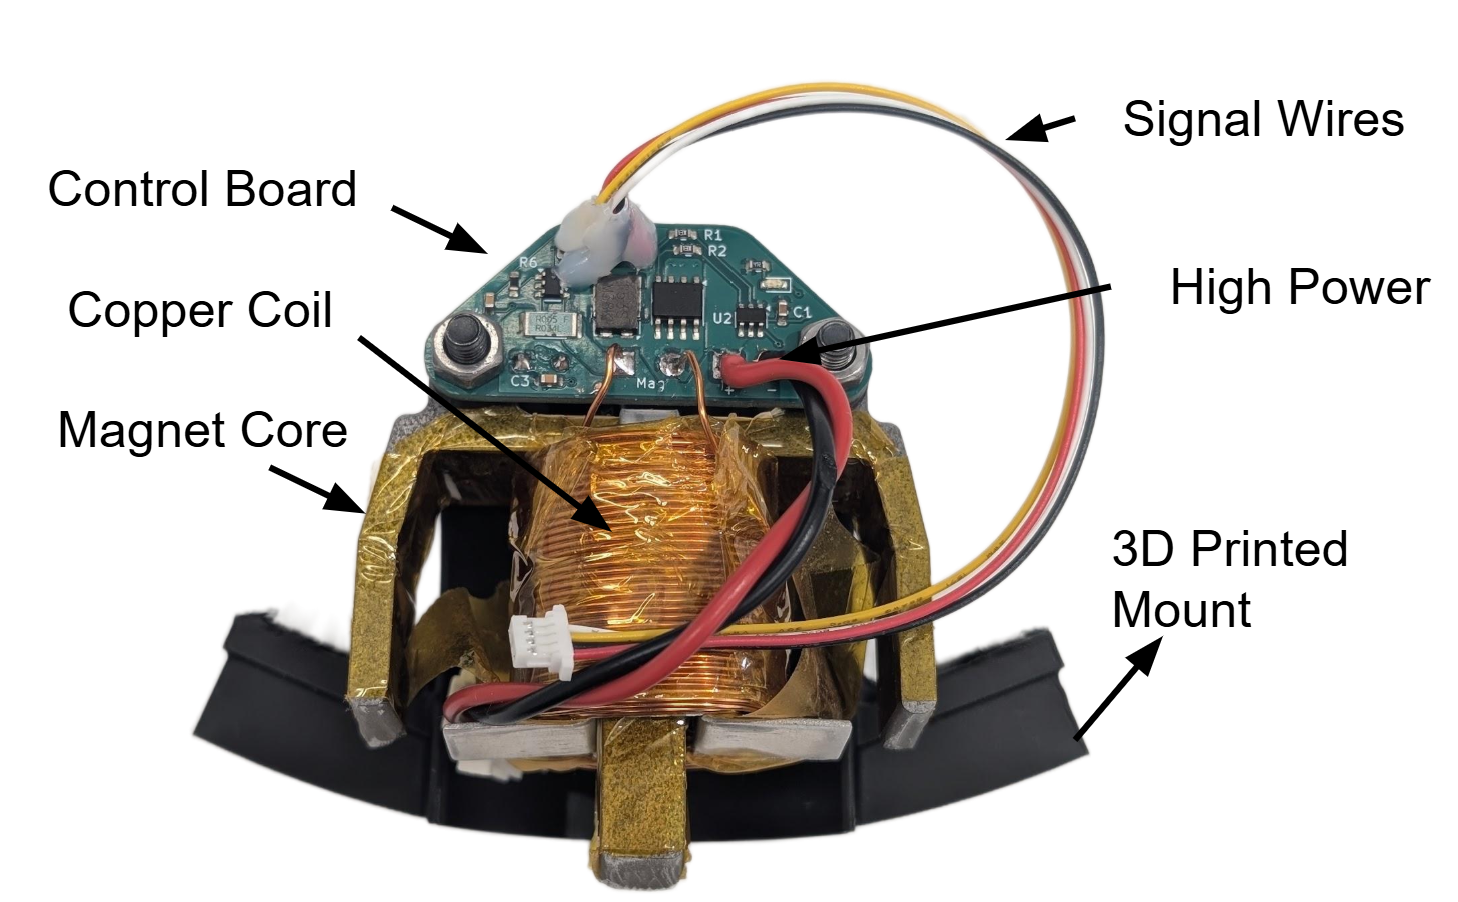
\includegraphics[width=0.8\textwidth]{Diagrams and Images/unit_cell.png}
    \caption[Unit Cell]{A completed electromagnet consisting of the steel core and copper coil, driving circuit board with signal and power connectors, and 3D printed mount.}\label{fig:unit_cell}
\end{figure}

\subsubsection{Icosahedral Geometry and Split Plane Design}
Maintaining spherical symmetry in our design was critical. Rotational inertia, available torque generation, and control complexity are simplified when the system behaves the same in all orientations. From our previous work, and magnet design testing, we found that the magnets were only effective when they were rotated to within 45 degrees of the steel plate. These requirements led us to a icosahedral geometry which has twenty faces that are equally spaced around the surface, with 42 degree angles between magnet centers. This allows us to place one magnet at the center of each face. We designed the sphere to be split into two hemispheres along a edge of the icosahedron, ensuring that no magnets are located on the split plane. This design choice allows for access to the internal components without the need to remove any magnets. See figure~\ref{fig:split_plane} for an image of the split plane design and how the two halves of the sphere combine.

\begin{figure}[h]
    \centering
    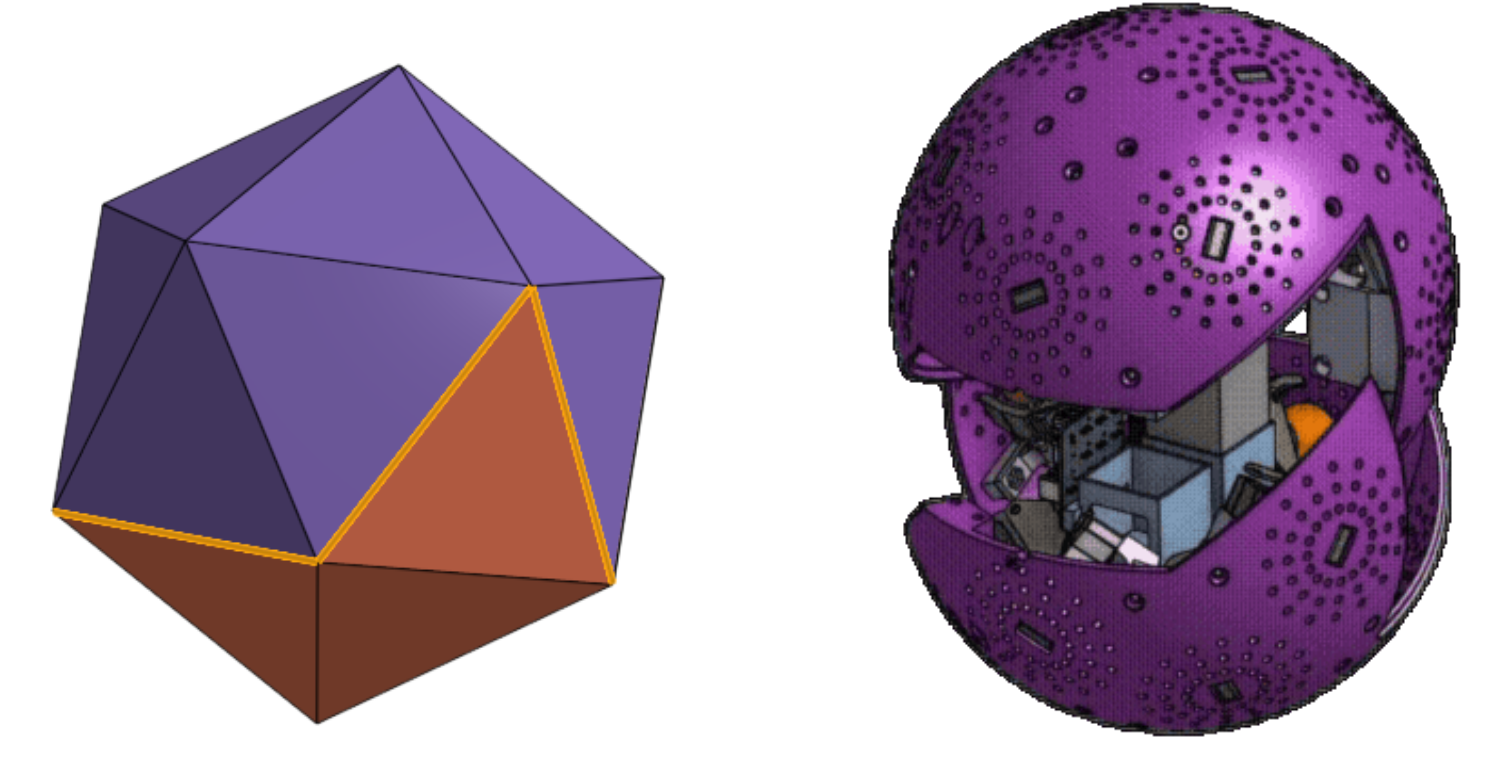
\includegraphics[width=0.8\textwidth]{Diagrams and Images/split_plane.png}
    \caption[Split Plane Design]{The sphere is designed to be split into two halves along a plane that does not intersect any magnets, allowing for easy assembly and maintenance.}\label{fig:split_plane}
\end{figure}

\subsubsection{Integration}
To connect the electromagnet boards to the microcontroller and power supply, four PCBs were designed and built. The power distribution boards take the main power supply and distribute it to the twenty electromagnet boards, while the signal distribution board takes the microcontroller’s control signals and routes them to the appropriate electromagnet boards. The main microcontroller board had three eight-channel analog to digital converters (ADCs) which read the current sense amplifier outputs and multiplex the signals to send to the microcontroller. Additionally, two sixteen-channel PWM drivers control the gate drivers, with ten magnets per driver. The ADCs use SPI protocol and scan all of the input signals, while the PWM drivers used the I2C protocol to communicate with the microcontroller. The microcontroller board also connected to an IMU board using I2C.


\section{Conclusion}
The primary objective of this project was to develop a three-dimensional spherical robot, capable of moving using the forces generated by interal electromagnets. By successfully integrating twenty individually controlled electromagnets, with a battery supply, IMU and microcontroller, we have proven that internal electromagnetic propulsion is a viable method for achieving motion along a steel surface. The successful implementation of the state machine algorithm demonstrates that the system can perform the complex, real-time orientation calculations required to activate the correct electromagnets for sustained movement.

While this prototype successfully validates the core mechanical, electrical, and software architecture of the robot, the current design faces a performance bottleneck. To achieve faster movement and responsive control, the intertia of the system must be addressed. Future development must focus on optimizing the power-to-weight ratio through the integration of higher-capacity batteries and increasing the number of magnets to achieve a finer resolution where more magnets are closer to the plate. The magnet activation algorithm can also be further refined as the current implementation does not factor in the rotational inertia of the ball.

\section{Recommendations}
The transition from the disk to a spherical robot introduces substantial design complexity, particularly in mechanical integration, control, and power systems. To support this next stage of development, we recommend the following key actions:

\textbf{Develop a 3D-Symmetric Electromagnet Design}\\
The trident geometry was optimized for planar motion in the disk prototype. For spherical implementation, the electromagnet design should be revised for three-dimensional symmetry to ensure consistent torque generation in all orientations. A proposed 3D design is included in Figure \ref{fig:three_images} (Appendix \ref{Spherical Images Appendix}).

\textbf{Integrate Optocoupleers and Redesign Driving PCBs}\\
To protect microcontroller signals from high-power switching noise, optical isolation should be integrated into future PCB designs. A PCB will improve reliability and simplify assembly.

\textbf{Design Modular Spherical Housing}\\
Each electromagnet functions as an independent subsystem. We recommend designing a modular spherical housing with magnets arranged in an icosahedral geometry (20 faces), which has uniform coverage and ease of assembly or replacement.

\textbf{Investigate Power Supply Instability}\\
Although motion control currently performs as expected, the power supplies exhibit unstable behavior. Diagnosing and resolving this issue—potentially caused by inrush currents, back EMF, or insufficient filtering—will be critical for safe and reliable operation.

\textbf{Model Electromagnet Positions and Orientations}\\
 Developing a 3D model of magnet positions and orientations will support integration with onboard IMUs and improve closed-loop control in three-dimensional motion.

\section{Deliverables}
\begin{enumerate}
    \item Github Repository
    \item Disk with Four Electromagnets on Optical Stand
    \item OnShape CAD Files
    \item KiCAD Circuit Schematic
\end{enumerate}

\begin{thebibliography}{9}

\bibitem{2507_report} 
Josh Bauman, Logan Underwood, Kristopher Kirkwood, Levi Varsanyi, Lucas Henderson, \textit{Project 2507: ELECTROMAGNETIC SPHERICAL ROBOT}, UBC Engineering Physics Project Lab, 2025.

\bibitem{Jenkins}
Jenkins, J. (2013, January 25). \textit{A closer look at switched reluctance motors.} Charged EVs. Retrieved April 8, 2025, from https://chargedevs.com/features/a-closer-look-at-switched-reluctance-motors/

\bibitem{ChatGPT}
OpenAI. (2025). \textit{ChatGPT} (April 6, 2025). https://www.openai.com/chatgpt

\bibitem{Hamraoui_2018}
Hamraoui, K., Van Damme, L., Mardesic, P. \& Sugny, D. (2018, March 16). \textit{(Color online) Definition of the Euler angles used to describe the position of the body-fixed frame.} ResearchGate. Retrieved April 10, 2026, from \url{https://www.researchgate.net/figure/Color-online-Definition-of-the-Euler-angles-used-to-describe-the-position-of-the_fig1_323821605}

\bibitem{Madgwick_2010}
Madgwick, S. O. H. (2010, April 30). \textit{An efficient orientation filter for inertial and inertial/magnetic sensor arrays.} University of Bristol. Retrieved April 10, 2026, from https://web.enib.fr/\textasciitilde kerhoas/iot/reseau-de-capteurs/carte-imu-mpu9250/documents/INVENSENSE/madgwick\_internal\_report.pdf


\end{thebibliography}
\newpage

\appendix
\setcounter{section}{0}  % Reset section counter

\section{Spherical Magnet Geometry}
\label{Spherical Images Appendix}
\begin{figure}[ht]
    \centering
    \begin{minipage}{0.3\textwidth}
        \centering
        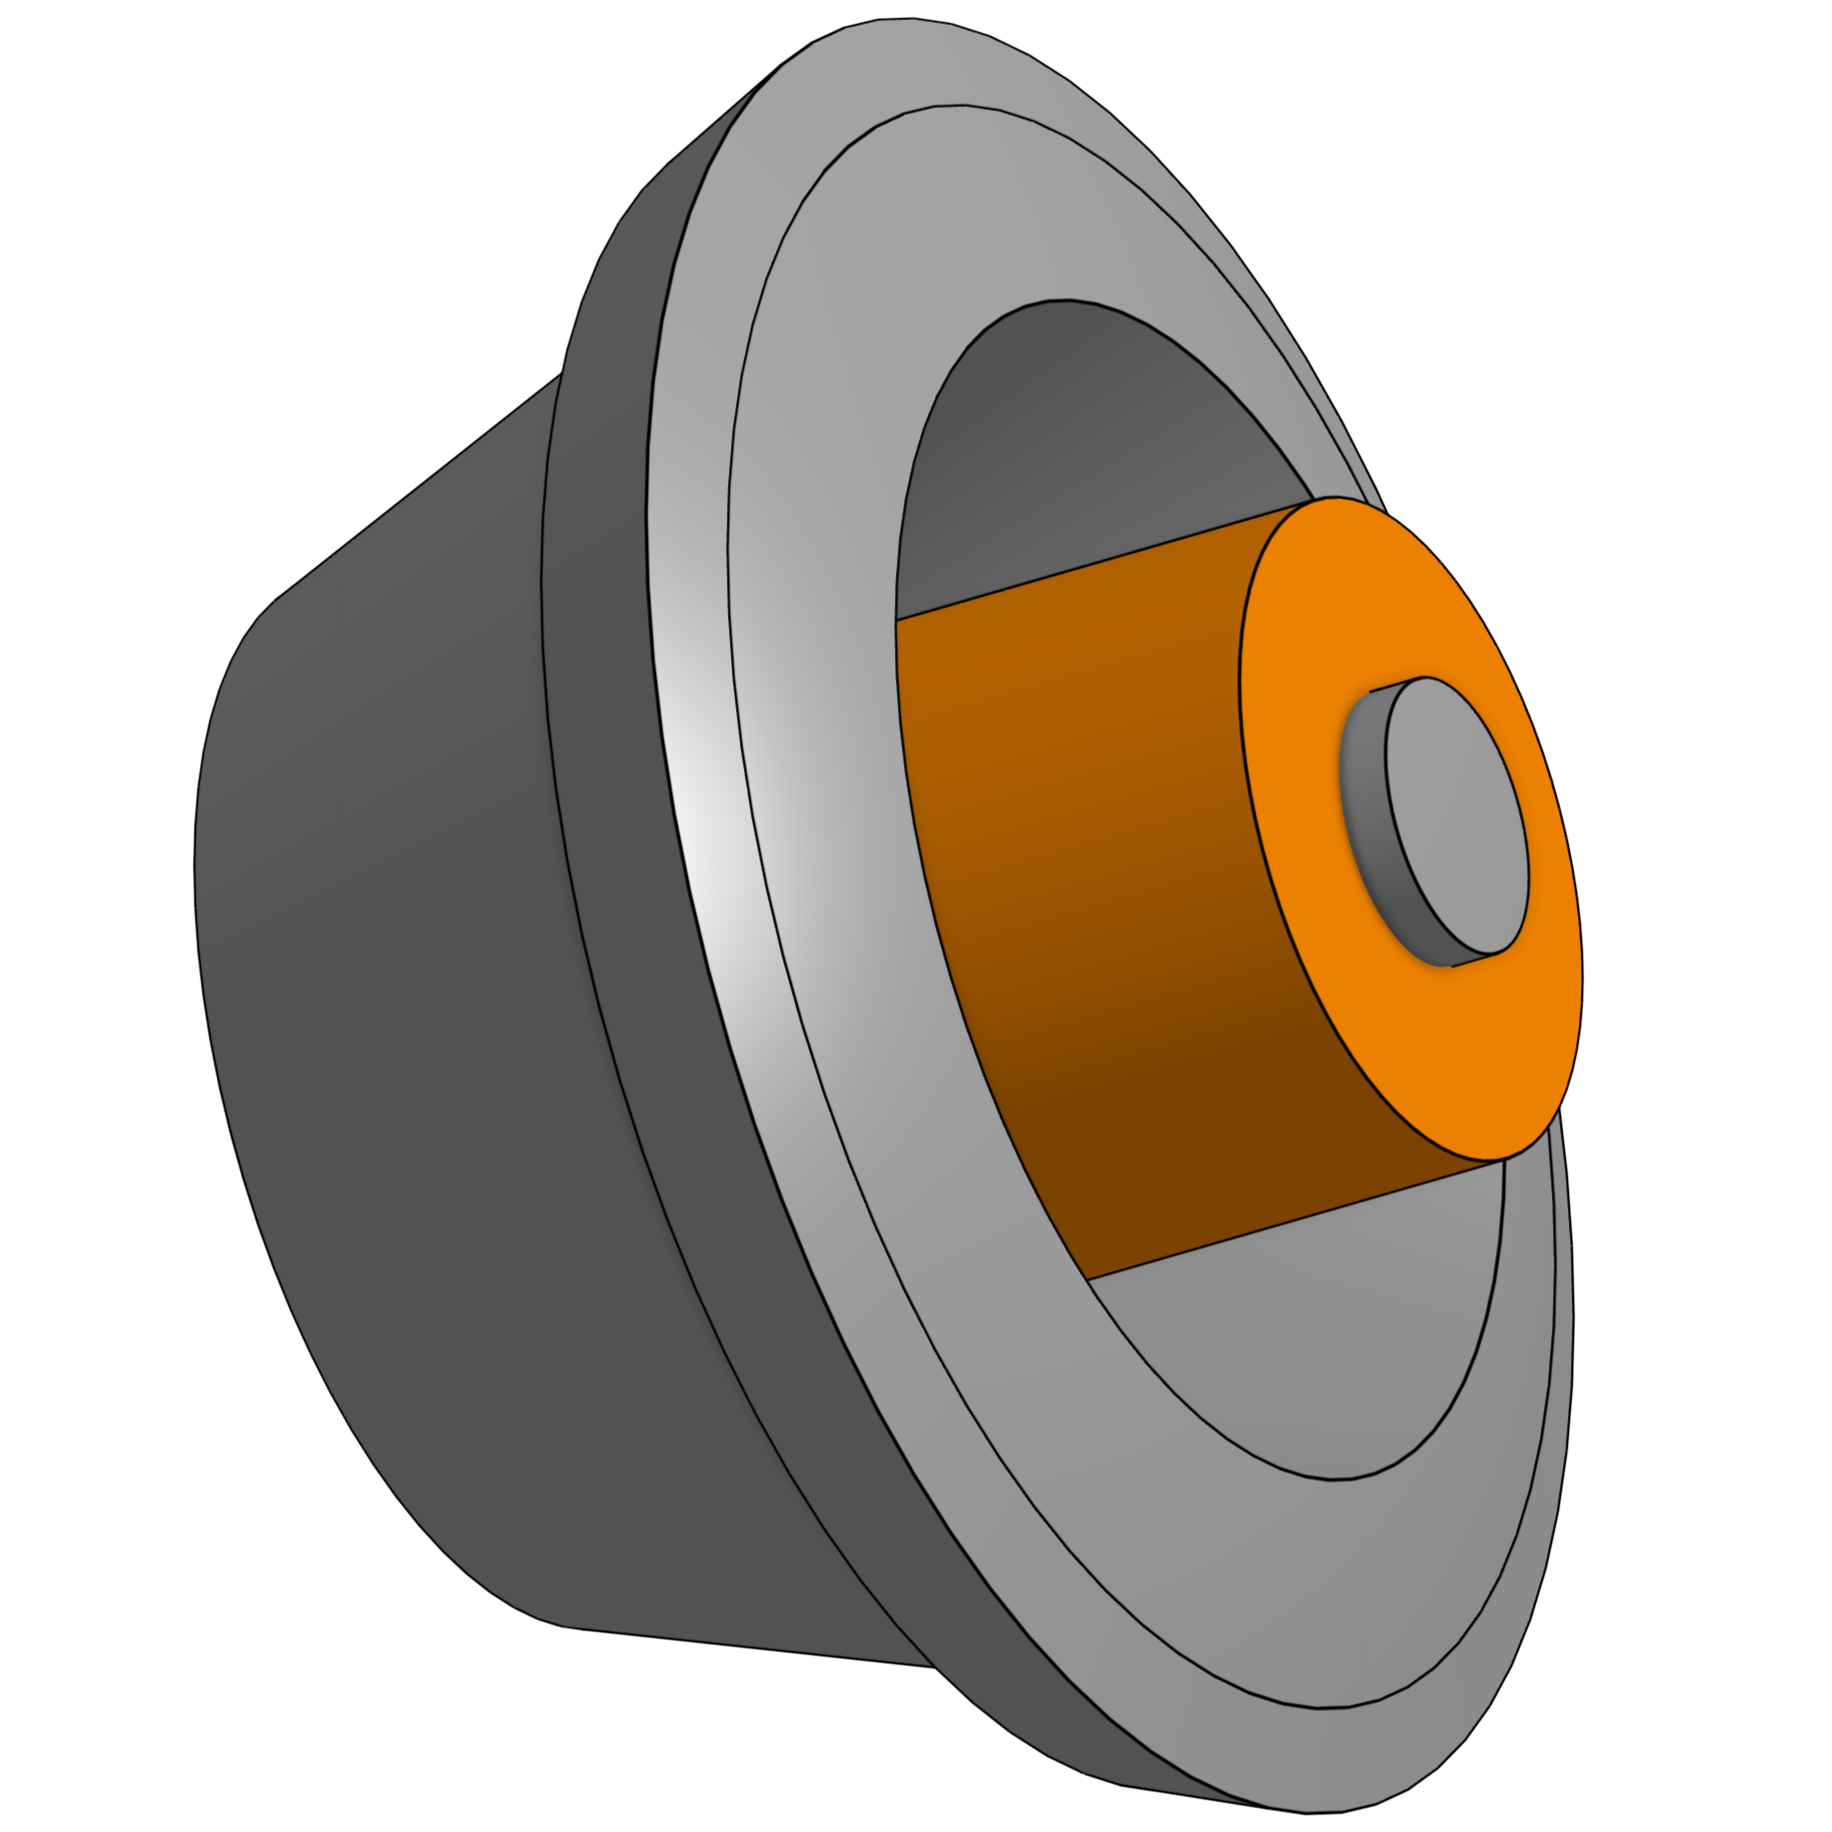
\includegraphics[width=\textwidth]{Kris_Visuals/3D Magnet Angle.png}
        \caption*{}  % Empty caption for the first image
    \end{minipage} \hfill
    \begin{minipage}{0.3\textwidth}
        \centering
        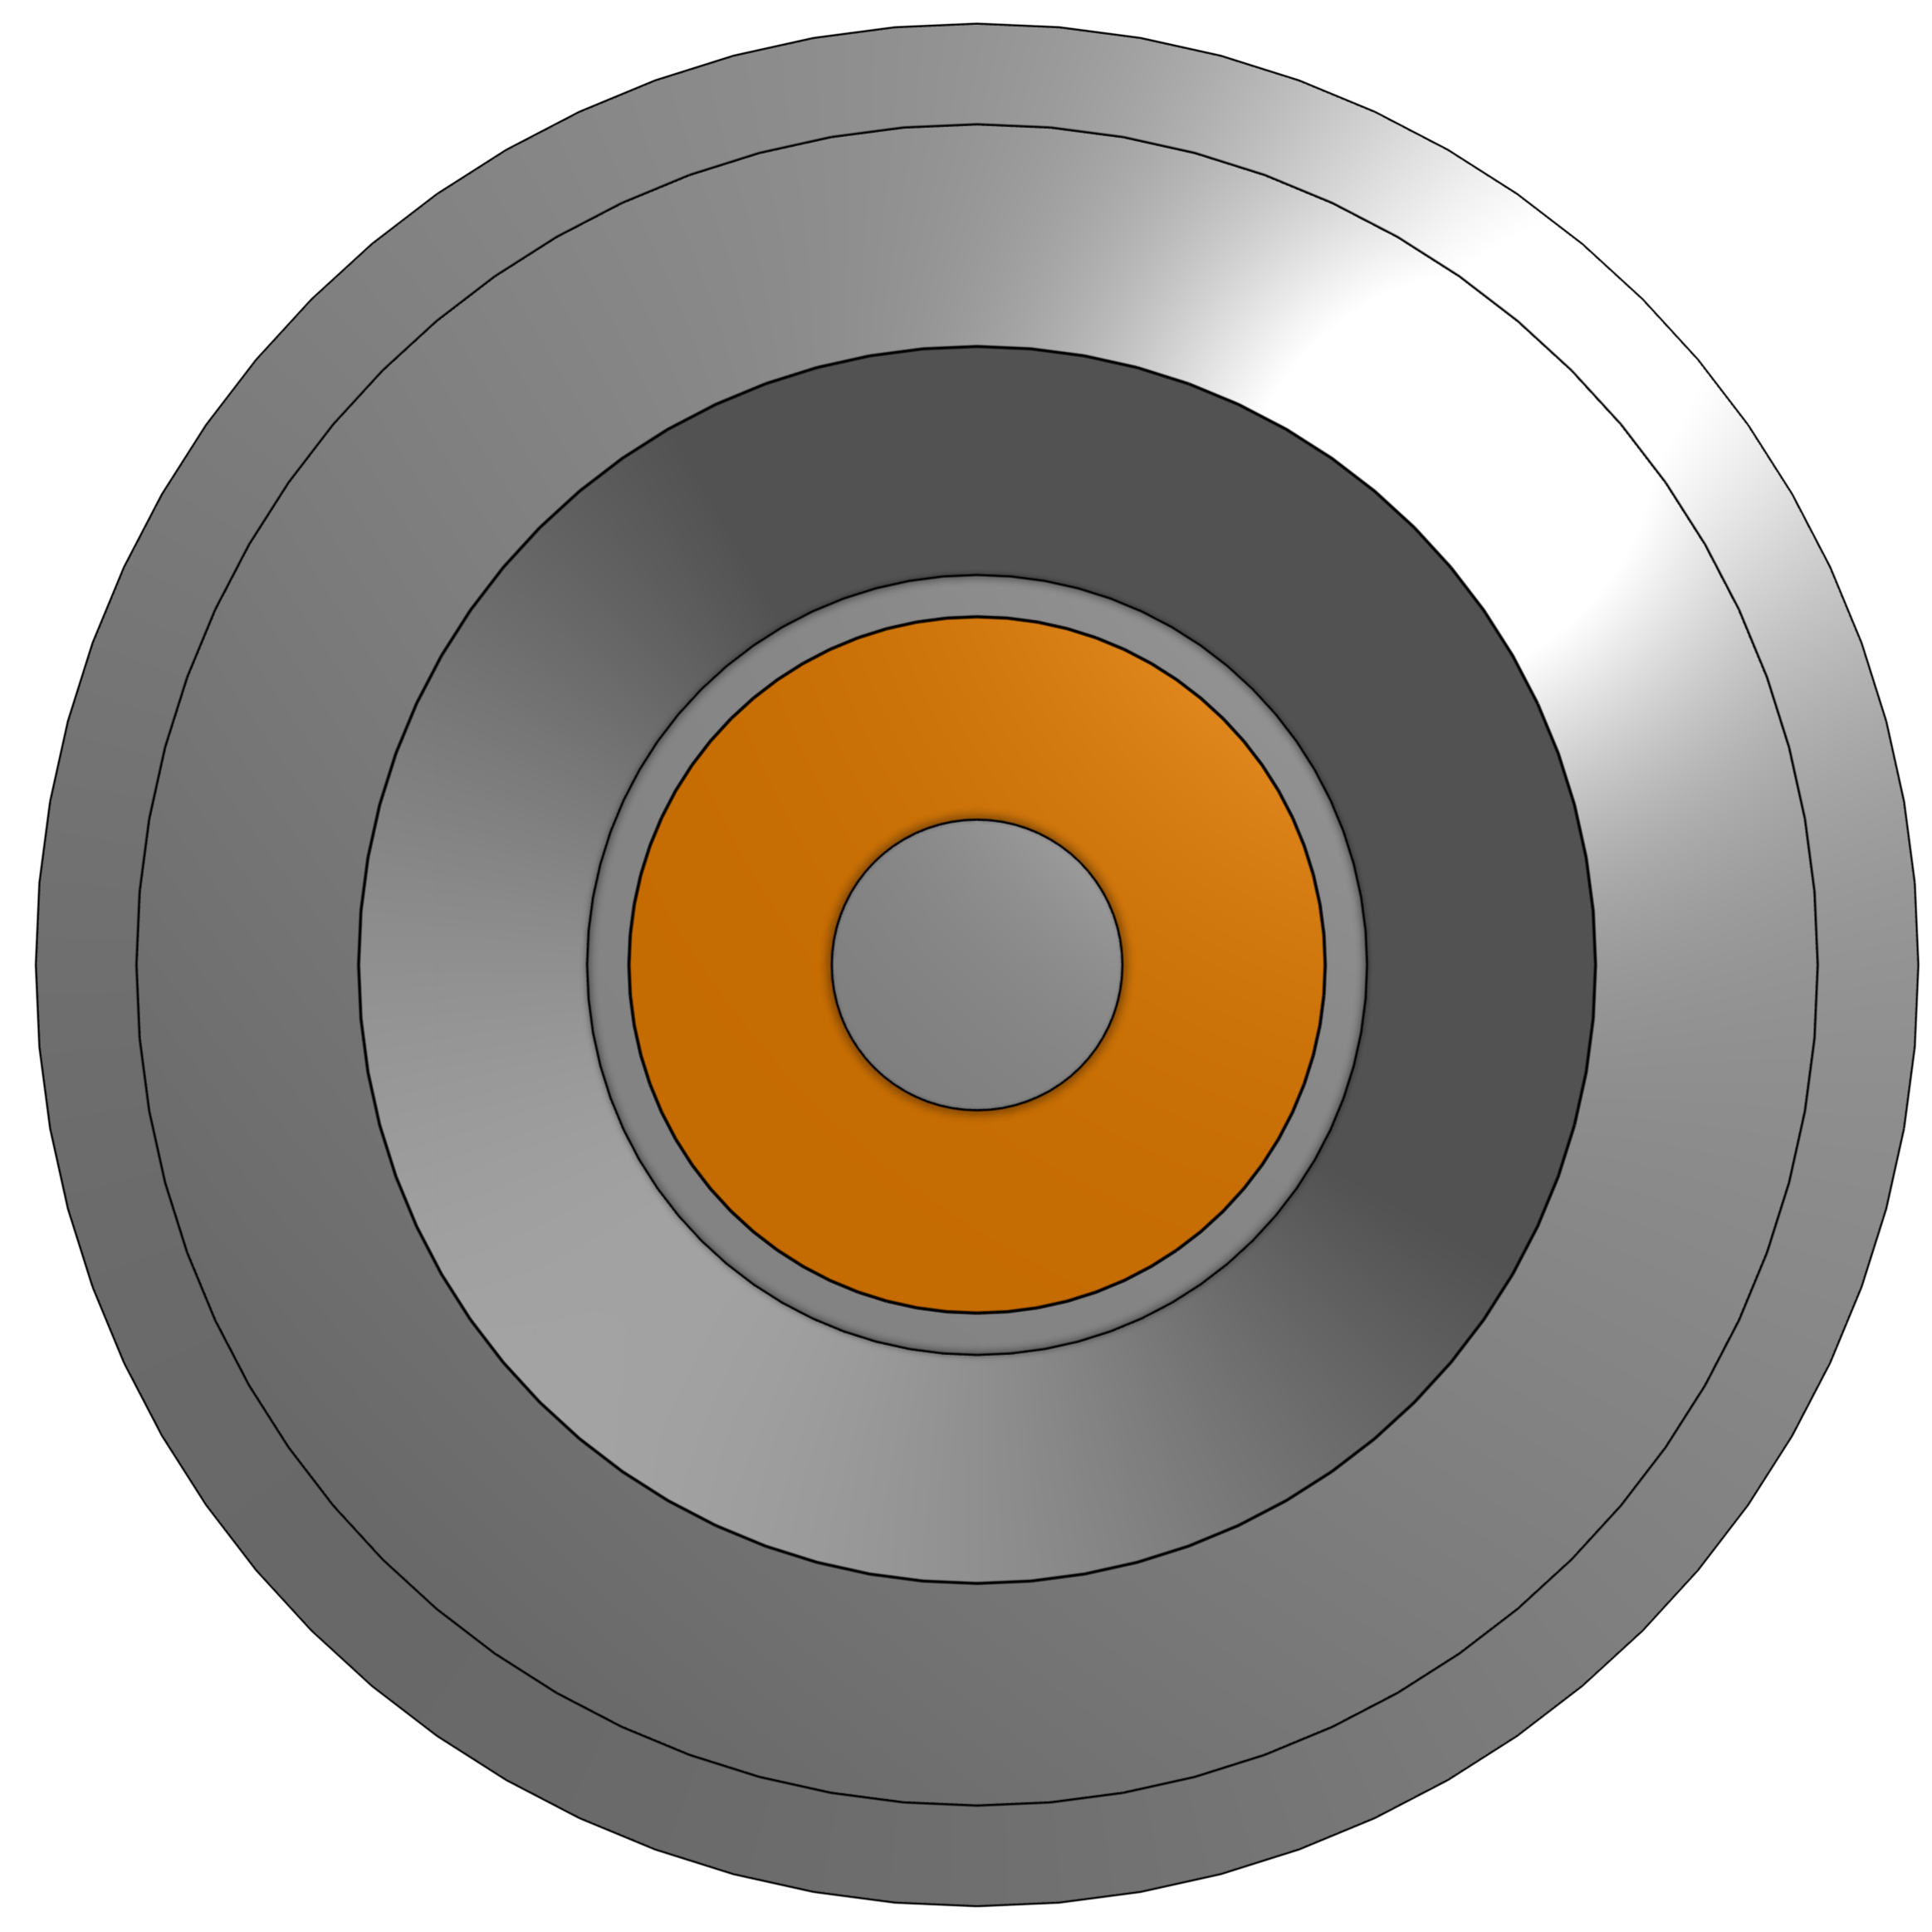
\includegraphics[width=\textwidth]{Kris_Visuals/3D Magnet Front View.png}
        \caption*{}  % Empty caption for the second image
    \end{minipage} \hfill
    \begin{minipage}{0.3\textwidth}
        \centering
        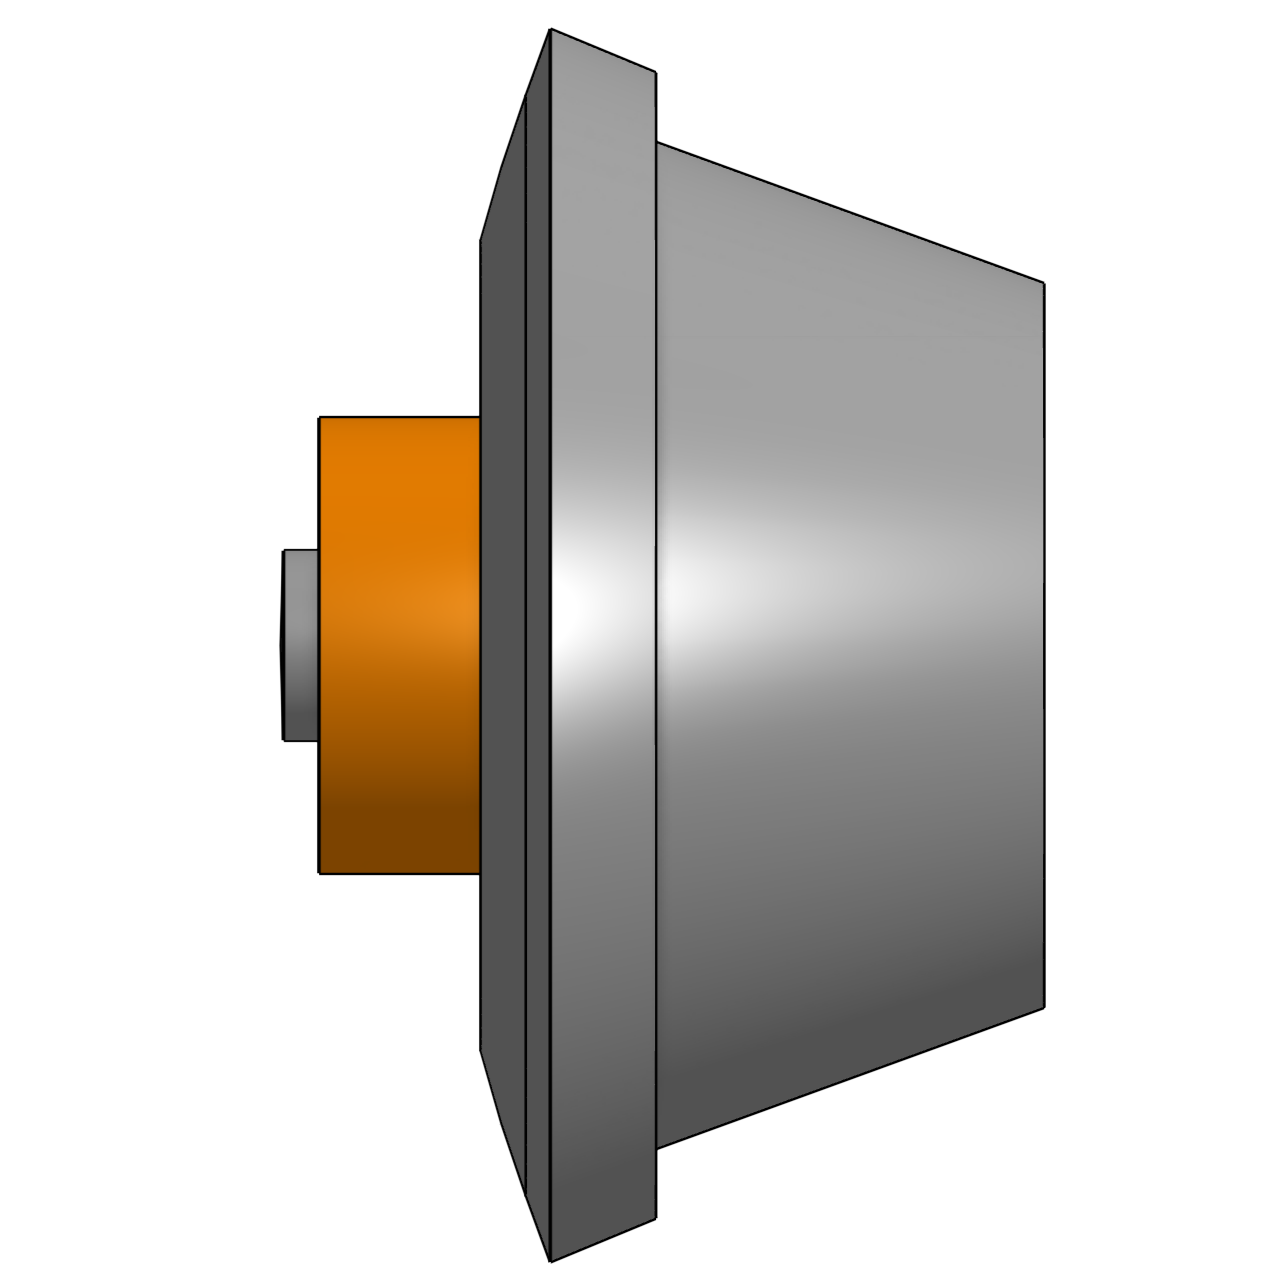
\includegraphics[width=\textwidth]{Kris_Visuals/3D Magnet Side View.png}
        \caption*{}  % Empty caption for the third image
    \end{minipage}
    
    \caption[Spherical Electromagnet Design Concept]{Spherical Electromagnet Design Concept}
    \label{fig:three_images}
\end{figure}

% \newpage
% \section{Current Sense Amplifier Datasheet}
% % \includepdf[pages=1,3,6,7,10,13,15]{Datasheets/av02-0956en.pdf}

% \newpage
% \section{Gate Driver Datasheet}
% \includepdf[pages={1,4,5,6,9}]{Datasheets/ucc27424.pdf}

% \newpage
% \section{MOSFET Datasheet}
% \includepdf[pages={1,5}]{Datasheets/Infineon-IRFZ44N-DataSheet-v01_01-EN.pdf}

% \newpage
% \section{Diode Datasheet}
% \includepdf[pages={1,2}]{Datasheets/sbx3040-3g.pdf}

\end{document}
